%\documentclass[twocolumn,pre,showpacs]{revtex4-1}
\documentclass[pre,showpacs]{revtex4}
\renewcommand{\baselinestretch}{2}
%\documentclass{nature}
%\bibliographystyle{naturemag}
\usepackage[pdfpagemode=None,pdfstartview=FitH]{hyperref}
\usepackage{graphicx}
\usepackage{hyperref}
\usepackage{epstopdf}
\usepackage[usenames]{color}

\def\br{{\bf r}}
\def\bu{{\bf u}}
\def\bw{{\bf w}}
\def\vcmi{v_{cm,i}}

\begin{document}

\title{Polymer Dynamics Across many regimes}

\author{Matthew Brunner}
\author{J.M. Deutsch}
\affiliation{Department of Physics, UCSC}
%My Vacuum polymer paper

\section{Introduction}

Polymer chains in a vacuum have been shown to have great importance
in many experimental situations, most often in application to mass
spectroscopy techniques that utilize the desorption of proteins into a vacuum. The
ability to desorb very large molecules without compromising their
integrity has many uses in biology~\cite{Hillenkamp}. Understanding
the statistical mechanics of such systems may help to improve current
spectroscopic techniques by providing information about other quantities,
aside from mass, that may be usefully measured. Aside from other
applications~\cite{DeutschPolyVac}, there is also the intrinsic interest
in understanding such systems. 

The dynamics of vacuum polymers has been the subject of a number of recent
investigations~\cite{Kleinert,mossa,DeutschPolyVac,DeutschCerf,Taylor,DeutschExactVac}  and show
many unusual features different from what are seen in solution. Polymers close to the coil-globule
transition show small Lyapunov exponents~\cite{mossa}. However in many situations,
the dynamics are in accord with detailed microcanonical calculations,
implying that these systems are ergodic~\cite{Taylor}. Ideal chains show
highly oscillatory time correlation functions~\cite{DeutschPolyVac}, whereas
the addition of self interactions damps these oscillations although they
are still quite pronounced for small chains~\cite{Taylor}.  Although there
is no coupling to a heat-bath, the nonlinear dynamics of these models
gives rise to an effective damping of individual monomers which is similar
to that of Kelvin damping~\cite{SethnaBookKelvinFriction}.  Adding local angular 
potentials to polymers increases this type of damping but does not
inhibit oscillations for sufficiently long chains~\cite{DeutschCerf}.

In this paper, we further investigate the equilibrium statistics
of a noninteracting polymer chain of $N$ links in a vacuum, where
energy, momentum, and angular momentum are conserved. Previous
work~\cite{DeutschExactVac} found an analytical solution for a ring
polymer with conserved angular momentum.  The average radius of gyration
as a function of angular momentum was obtained. The most
surprising feature of that calculation is that the radius of gyration when
the angular momentum is zero is less than that of a chain without that
conservation law. The radius of gyration still is proportional
to $\sqrt{N}$ but now with a different proportionality constant.

The calculation performed for a ring chain~\cite{DeutschExactVac} does not
extend easily to linear chains.  Here we use an approach that diverges considerably
from the previous one to obtain the statistics of a linear chain under
the same conditions. The new approach has some similarities to techniques used in statistical quantum mechanics~\cite{KleinertBook}In both cases, although the intermediate steps
produce rather lengthy expressions, the final answers are quite simple.
This suggests that there may be another underlying principle that can be
used to understand systems with constant angular momentum.

Aside from the average radius of gyration of such a system, there is
another important quantity that describes it, that has hitherto not
been studied. For finite angular momentum, the chain is expected to
become anisotropic, flattening in the direction of the angular momentum
vector. It is therefore of interest to calculate the average size
of a chain both perpendicular and parallel to the angular momentum.
However our analytic method is only applicable in calculating quantities
which have rotational symmetry such as the radius of gyration. It will
not work for studying chain anisotropy. Therefore we turn to numerical
methods to study this problem. We find, rather surprisingly, that the
chain continuously flattens in the direction of the angular momentum
showing universal scaling in the same rescaled variables used to
characterize the full radius of gyration. 



\section{Exact Solution}
Following previous work ~\cite{laliena} we begin by writing down the entropy as a function of the total energy $E$, angular momentum $L$, and number of particles $N$,  including terms for the conservation laws to be enforced. 
\begin{equation}
W(E,L,N) = C \int \delta(E - K - \Phi)\delta^{(3)}(\mathbf{L} - \sum_i \mathbf{r}_i \times \mathbf{p}_i)\delta^{(3)}(\mathbf{r}_{cm})(\prod_{i=1}^N d^3r_id^3p_i)
\end{equation}
where $K$ is the total kinetic energy and $\Phi$ the total potential energy. We are choosing a coordinate system so that
the center of mass $\mathbf{r}_{cm} = 0$.

We take the potential energy to be the elastic energy of the polymer chain and in addition include an isotropic quadratic potential that
will be used to calculate the radius of gyration. In terms of the continuous arclength $s$ dependent position variables that we will use 
below, 
\begin{equation}\label{eq:DefPhi}
\beta \Phi =  \int^{Nl}_0 \frac{3}{2l} |\frac{d \mathbf{r}}{ds}|^2 + \epsilon r^2(s)  ds 
\end{equation}
where $l$ is the chain link length, which is independent of the other properties of the chain.

Because we are taking $N$ to be large, we can convert this to a partition function, with the energy conserving delta function expanded in exponential form.
\begin{equation}
Z(\beta,L,N) \propto  \int d^3k \int e^{ i\mathbf{k\cdot L} }e^{ -\beta(K+\Phi) }e^{ -i\mathbf{k}\cdot \sum_i \mathbf{r}_i\times \mathbf{p}_i }\delta^{(3)}(\mathbf{r}_{cm})(\prod_{i=1}^N d^3r_id^3p_i)
\end{equation}

After integrating over the momenta and taking into account rotational symmetry we arrive at the form~\cite{DeutschExactVac}

\begin{equation}\label{partzeta}
Z[\beta,L,N] = \frac{c}{L} \int_0^\infty \sin(kL)\zeta(\beta,k)dk
\end{equation}
where $\zeta$ is a function of the magnitude of $k$ and inverse temperature  $\beta$ only. The constant $c$ is of no physical importance and
\begin{equation}\label{rawzeta}
\zeta(\beta,k)= \int e^{ -\int^{Nl}_0 (\frac{Tmk^2}{2l} +\epsilon)(x(s)^2 + y(s)^2)+\epsilon z(s)^2 + \frac{3}{2l}  |\dot{\mathbf{r}}|^2  ds}\delta(\mathbf{r}_{cm}) \delta \mathbf{r}(s) .
\end{equation}
Now we perform a scaling on $L$, $k$, and $s$ in order to normalize out the length of the chain and the temperature.
\begin{eqnarray}
L^\prime = \frac{\sqrt{12}}{Nl\sqrt{mT}} L\\
k^\prime = \frac{Nl\sqrt{mT}}{\sqrt{12}} k\\
s^\prime = \frac{\sqrt{12}}{Nl} s
\end{eqnarray}
The rescaling factors are based on the expected value of $L$ for the usual model without conservation of angular momentum, and produce a set of dimensionless variables. This will allow us to compare chains of all sizes and temperatures on a common scale.
After doing these rescalings, the form of Eq. \ref{partzeta} remains unchanged, and Eq. \ref{rawzeta} changes to:
\begin{equation}\label{scaledzeta}
\zeta(\beta,k^\prime)= \int e^{-\int_0^{\sqrt{12}} (k^{\prime2}/2l + \epsilon^\prime)(x^\prime(s^\prime)^2 + y^\prime(s^\prime)^2 ) + \epsilon^\prime z^\prime(s^\prime)^2  + \frac{3}{2l} |\dot{\mathbf{r}^\prime}|^2 ds^\prime}\delta(\mathbf{r}^\prime_{cm}) \delta \mathbf{r^\prime}(s^\prime)
\end{equation}
It is interesting to note that the explicit dependence on $\beta$ has disappeared and $\zeta$ is now only a function of $k^\prime$. The dependence on the total length of the chain has also been factored into $k^\prime$, but the length of the individual monomers remains.
Now we expand the center of mass conserving delta function in complex exponential form.
\begin{equation}
\zeta(k^\prime)= \int e^{-\int_0^{\sqrt{12}} (k^{\prime2}/2l + \epsilon^\prime)(x^{\prime2} + y^{\prime2} ) + \epsilon^\prime z^{\prime2}  + \frac{3}{2l} |\dot{\mathbf{r}^\prime}|^2 + i x^\prime l_x + i y^\prime l_y + i z^\prime l_z ds^\prime}  dl_xdl_ydl_z \delta \mathbf{r^\prime}(s^\prime) .
\end{equation}
These terms can be combined with the existing exponents using completion of squares which results in path independent phase factors and a constant offset to the paths, e.g. $x^\prime (s) \to x^\prime (s) + const.$ . Since all possible paths are included in the integral, the offset has no effect.

We now have a nice separation into a simple Gaussian integral and a factor that is very similar to the path integral form of a harmonic oscillator. 
\begin{equation}
(\int e^{\sqrt{12}[ -(l_x^2 + l_y^2)/4(\frac{k^{\prime2}}{2l} +\epsilon^\prime) - l_z^2/4\epsilon^\prime]}dl_xdl_ydl_z)  (\int e^{-\int_0^{\sqrt{12}} (k^{\prime2}/2l + \epsilon^\prime)(x^{\prime2} + y^{\prime2} ) + \epsilon^\prime z^{\prime2}  + \frac{3}{2l} |\dot{\mathbf{r}^\prime}|^2 } \delta \mathbf{r}^\prime)
\end{equation}
The first integrals of the $l$'s are trivially integrated but we must still perform the path integral in parentheses. 
These decouple into path integrals over the $x$, $y$, and $z$ directions and each one has an action of the form
\begin{equation}
\int_0^{\beta_0} \frac{M}{2}(\dot{x}^2 + \omega_0^2 x^2)dt .
\end{equation}
$M$ does not depend on $k$ or $\epsilon$, and $\omega_z$ has no $k$ dependence.
After making this analogy, we can see that for any two fixed path endpoints, the functional integration will give the Greens function for a thermal harmonic oscillator. To obtain a sum over all paths, we simply need to integrate the Greens function $\rho$ ~\cite{feynman} over both its arguments,
\begin{equation}
\zeta_i = \int \rho_i(x_1,x_2)dx_1dx_2
\end{equation}
where $i = 1,2,3$ represent the $x$, $y$, and $z$, path integrals respectively.
The Greens function is easily integrated and the result is 
\begin{equation}\label{eqn:zomega}
\zeta_i \propto \frac{\omega_i}{\sqrt{ \sinh{(\sqrt{12}\omega_i)}}}
\end{equation}
Putting all of this back into Eq. \ref{partzeta} we get the form for $Z$
\begin{equation}
Z(L^\prime) = \frac{c}{L} \sqrt{\frac{\omega_z}{\sinh{(\sqrt{12}\omega_z)}}} \int_0^\infty k^\prime \sin(k^\prime L^\prime) \frac{\omega}{\sinh(\sqrt{12}\omega)} dk^\prime .
\end{equation}
The radius of gyration can be expressed as
\begin{equation}
R_g^2 = -\frac{1}{Nl}\frac{\partial \ln Z}{\partial \epsilon}\vert_{\epsilon=0}
\end{equation}
The logarithmic derivative allows us to separate the factors in $Z$ and treat each as terms in a sum.
The first term is simple
\begin{equation}
\lim_{\epsilon\to0}\frac{\partial \ln}{\partial \epsilon}\sqrt{\frac{\omega_z}{\sinh{(\sqrt{12}\omega_z)}}} = -\frac{1}{18}N^2l^3
\end{equation}
The second term is more complex due to the integral, so we begin by rewriting the logarithmic derivative as a ratio.
\begin{equation}
\lim_{\epsilon\to0} \frac{\frac{\partial}{\partial \epsilon}\int_0^\infty k^\prime \sin(k^\prime L^\prime) \frac{\omega}{\sinh(\sqrt{12}\omega)} dk^\prime}{\int_0^\infty k^\prime \sin(k^\prime L^\prime) \frac{\omega}{\sinh(\sqrt{12}\omega)} dk^\prime}
\end{equation}
Since the integral is over $k^\prime$ we can pull the derivative and limit inside the integration. This simplifies the integrand considerably as $\lim_{\epsilon\to0} \omega = k^\prime/\sqrt{3}$
\begin{equation}
\lim_{\epsilon\to0} \frac{\frac{\partial}{\partial \epsilon}\int_0^\infty k^\prime \sin(k^\prime L^\prime) \frac{\omega}{\sinh(\sqrt{12}\omega)} dk^\prime}{\int_0^\infty k^\prime \sin(k^\prime L^\prime) \frac{\omega}{\sinh(\sqrt{12}\omega)} dk^\prime}  = \frac{L^\prime N^2}{6\pi l^3\tanh(\frac{L^\prime \pi}{4}) }
\end{equation}
Putting all of these pieces together we obtain our final result,
\begin{equation}
\label{eq:finalresult}
\frac{R_g^2}{Nl^2} = \frac{1}{18} + \frac{L^\prime}{6\pi\tanh(\frac{L^\prime\pi}{4})}
\end{equation}
A plot of this is shown in Fig. \ref{fig:rgplot} by the solid line. The simulation results that are also displayed will be discussed in Sec. \ref{sec:simresults}.
Note that for $L^\prime = 0$, $R_g^2/(N l^2) = (1/18) + 2/(3 \pi^2) \approx 0.1231$, which is about $74\%$ of $1/6$, the value of the same
quantity without conservation of angular momentum enforced.
\begin{figure}
\begin{center}
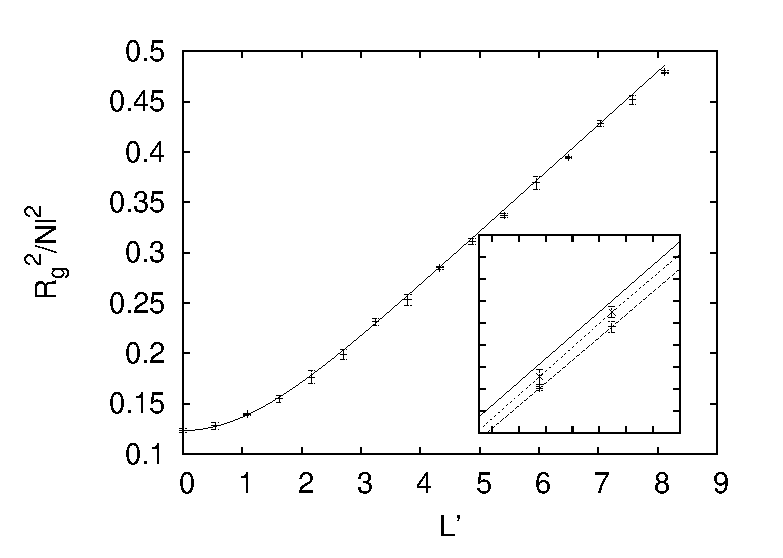
\includegraphics[width=\hsize]{radius}
\caption{Plot of $\frac{R_g^2}{Nl^2}$ along with simulation results
using a chain length $N = 128$. Inset is a section from $L^\prime=5.5$
to $L^\prime=7$ showing the exact solution as a solid line along with results from simulations done with $N = 32$ (farthest from line)
and $N = 64$. }
\label{fig:rgplot}
\end{center}
\end{figure}

For the same reason as for the ring calculation~\cite{DeutschExactVac}, for fixed $L^\prime$ and $N\to \infty$, we are permitted to take this
system to be at constant temperature, because as was discussed in detail~\cite{DeutschExactVac}, the relation between energy and temperature
has no dependence on $L^\prime$ in this limit.


\section{High $L$ limit}
In the limit of large $L$, Eq. \ref{eq:finalresult} gives $R_g^2/Nl^2 \to L^\prime/6\pi$. One would expect typical configurations at high $L$ would consist of a fairly straight line rotating rapidly around its center. The solution for the equilibrium case of constant angular velocity can be found by setting the change in tension along the chain equal to the centripetal force. This gives an equation for the position of each monomer as a function of its location along the chain, $r(s)$, for simplicity defined with $s=0$ at the center of the chain. For large $N$, the tension approaches zero at the ends of the chain.
\begin{equation}
-k\frac{d^2r}{ds^2} = m \omega^2 r \\
\end{equation}
where $k$ is the entropic elastic spring coefficient.
From this we get that $r(s) \propto \sin(\sqrt{\frac{m}{k}}\omega s)$, and that $Nl\omega/2\sqrt{k} = \pi/2$. Higher modes exist, but they double back and are expected to not be minimal free energy solutions. They are also not consistent with the straight chain model we are assuming. Using the integral definition of angular momentum
\begin{equation}
L = \frac{m \omega}{l}\int_0^{Nl}  r^2(s)ds 
\end{equation}
the radius of gyration squared is
\begin{equation}
R_g^2 \equiv \frac{1}{Nl}\int r^2(s)ds = \frac{1}{\omega m N } L = \frac{1}{\sqrt{mk}\pi}L = \frac{l}{\sqrt{3mT}\pi}L = \frac{L^\prime Nl^2}{6\pi}
\end{equation}
and therefore we see that in the limit of high $L$, our model behaves as one would expect.
\section{Partition Function}
The partition function itself can be obtained easily from Eq. \ref{eqn:zomega} by taking $\epsilon \to 0$ and performing the integration.
\begin{equation}
\lim_{\epsilon \to 0} Z = \frac{1}{L} \int k^{\prime2} \frac{\sin(k^\prime L^\prime)}{\sinh(2k^\prime)}dk^\prime = \frac{\pi^3}{32L^\prime}\frac{\tanh(L^\prime \frac{\pi}{4})}{\cosh^2(L^\prime \frac{\pi}{4})}
\end{equation}
To obtain the distribution over $L^\prime$ we need to normalize this Z, taking in to account the angular integration over the direction of $L^\prime$.
\begin{equation}
\int 4\pi L^{\prime2} Z dL^\prime = \pi^2
\end{equation}
so our normalized partition function is 
\begin{equation}
Z = \frac{\pi}{32L^\prime}\frac{\tanh(L^\prime \frac{\pi}{4})}{\cosh^2(L^\prime \frac{\pi}{4})}
\end{equation}
A plot of this is displayed in Fig. \ref{fig:P}.
This partition function can be related to the probability density in the space of angular momentum. Since $Z$ was normalized for three dimensions, it will be the three dimensional density $\rho(\mathbf{L^\prime})d\mathbf{L^\prime}$. One can simply integrate out the trivial angular dimensions to get the density in terms of the radial scalar $L^\prime$.

The distribution shows a long exponential tail into high $L^\prime$.
\begin{figure}
\begin{center}
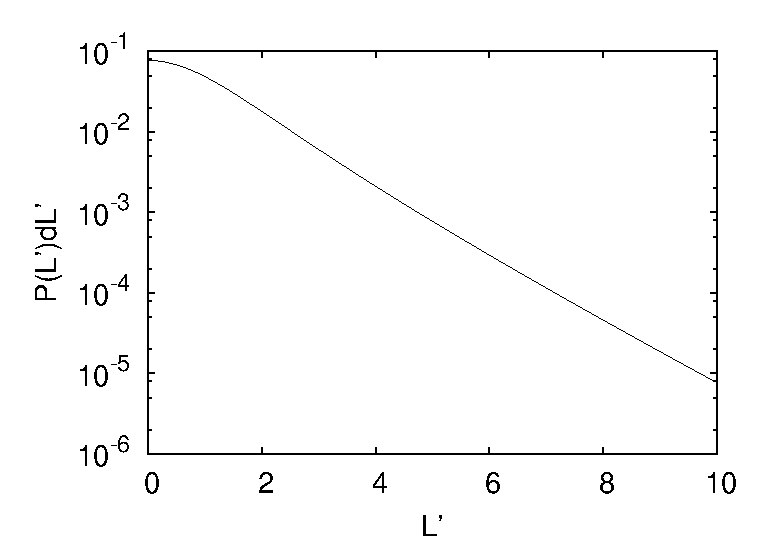
\includegraphics[width=\hsize]{P}
\caption{Plot of $P(L^\prime))$, with clear non-Gaussian behavior for high $L^\prime$}
\label{fig:P}
\end{center}
\end{figure}

\section{Simulation Results}
\label{sec:simresults}
In addition to the exact calculation, further studies were carried out using simulation. First the analytical results concerning the radius of gyration as a function of $L^\prime$ were verified. Second we were able to investigate other quantities that were beyond the means of our analytic method.

\begin{figure}
\begin{center}
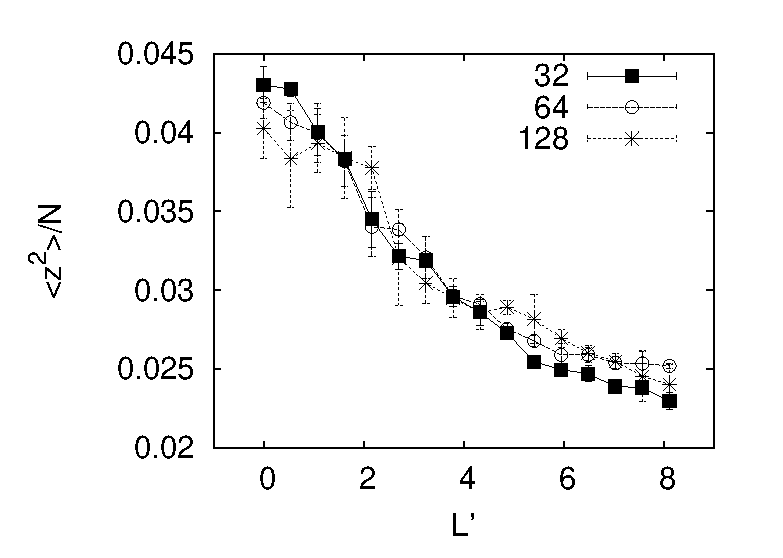
\includegraphics[width=\hsize]{zsq}
\caption{Plot of the simulated radius of gyration in the direction of angular momentum as a function of rescaled $L$, for chain sizes $N=32$,$64$ and $128$. }
\label{fig:zsq}
\end{center}
\end{figure}


We used a molecular dynamics method ~\cite{DeutschCerf} that was developed to simulate chains in a vacuum. It
consisted of freely rotating rigid links, conserving energy and angular
momentum, corresponding to a system with fixed temperature and angular momentum. Rigid links were employed to minimize problems with equilibration that are often seen with one dimensional nonlinear systems~\cite{FPU,BermanIzrailev}. The input angular momentum and the output measurements were
scaled by the total chain length for comparison. The initial values of
the angular momentum were chosen to cover a range of $L^\prime$ values, and the
angular momentum was explicitly checked and conserved during the runs.
First the simulation was compared to the theoretical results for the
normalized radius of gyration. The results of these simulations can be
seen in Fig. \ref{fig:rgplot}, and show excellent agreement with the
theoretical prediction. The main plot shows the exact result (solid line)
along with data for chains with $N=128$. The inset shows that the deviation in the asymptotic form for high
$L^\prime$ decreases as the number of simulation chain links is increased and
appears to be due to the finite size of the simulation system. The two chains lengths
used in the inset are $N=32$ and $N=64$ which are more accurate than the data
for $N=128$. They also indicate that the finite size corrections to the
analytic form are $O(1/N^\alpha)$ for some $\alpha$ of order unity, as shown in Fig. \ref{fig:scalen}.
\begin{figure}
\begin{center}
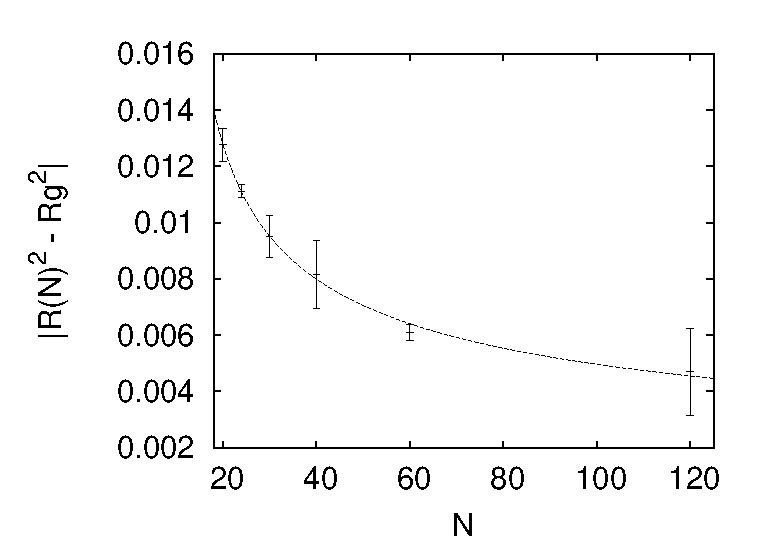
\includegraphics[width=\hsize]{scalen}
\caption{Plot of the deviations in $R_g^2$ as a function of chain size $N$. The dashed line is the best fit curve with $\alpha = 0.436$.}
\label{fig:scalen}
\end{center}
\end{figure}

For nonzero angular momentum the polymer chain is expected to become
anisotropic. The analytic methods used earlier require an isotropic
form for the quantities being averaged, causing the investigation
of the anisotropy by such means to be outside the scope of our
analysis. Therefore we turned to the simulation to explore the aspect
ratio of the polymer as a function of $L^\prime$, with the aspect ratio is defined
as $\sqrt{\langle z^2 \rangle /\langle R_g^2 \rangle}$. The aspect ratio
itself is dominated by the asymptotic linear behavior of the radius of
gyration, and displays what appears to be an inverse power law falloff
as expected. More interestingly, $\langle z^2 \rangle$ itself appears to
fall off as $L^\prime$ increases, even for low values of $L^\prime$.  This is shown in Fig. \ref{fig:zsq}  where the
vertical axis is scaled in the same manner as for the radius of gyration,
by dividing by $N$ and taking $l,m,T$ all to be unity, and the horizontal axis is $L^\prime$.  The three chain lengths seem to collapse onto one curve after the rescaling of length
and angular momentum. This is unexpected because for a ideal gaussian
chain each dimension has independent statistics, which our model should resemble for low $R_g$. The coupling should only be apparent in the limit of high $L$ where 
the rigid link model should approach a straight line solution. However
this is unlikely to be an explanation, as the straight line regime
would imply a leveling off of the radius of gyration, which is not
seen, see Fig. \ref{fig:rgplot}. Moreover, the falloff is independent of the number of chain links
in the simulation and collapsed onto a single curve, so is not likely
due to the non gaussian nature of the model. This decrease in $\langle z^2 \rangle$ is slow and
does not appear to have a nonzero asymptote, and is likely to be a low
power law or logarithmic in nature.


%For my own reference:
%\begin{eqnarray}
%\rho(x,x^\prime;U) = \int e^{-\frac{1}{\hbar}\int_0^U[\frac{m\dot{x}(u)^2}{2} + V(x(u))]du}dx(u) \\
%U = \beta\hbar \\
%\rho(x,x^\prime;\beta) = \sqrt{\frac{m\omega}{2\pi\hbar\sinh(\hbar\omega/kT)}}e^{ \frac{-m\omega}{2\hbar\sinh(\hbar\omega/kT)}[(x^2+x^{\prime2})\cosh(\frac{\hbar\omega}{kT}) - 2xx^{\prime2}] }
%\end{eqnarray}


\section{Conclusions}

In this paper, we considered the equilibrium properties of an ideal linear chain in a vacuum
that conserves energy, momentum, and angular momentum. We were able to compute the average
radius of gyration of such a chain as a function of its angular momentum $L$. We also computed
the distribution of angular momenta for chains in thermal equilibrium. 
We verified that our analytical result for the radius of gyration is correct by performing
numerical simulation and by analyzing its asymptotic form in the limit of large angular momentum.
The derivation of this result differs from that of a ring chain but in both cases the final
result is relatively simple involving hyperbolic trigonometric functions. The underlying reason
for this is still unclear.

Our numerical simulations show that the radius of gyration perpendicular
to the angular momentum vector increases with $L$, as to be expected,
however in addition to this, the radius of gyration parallel to the
angular momentum, which we take to be in the $z$ direction, decreases.
This is very different than what a naive analysis would suggest. If we
were to go to a frame rotating at angular velocity $\Omega$, then in
thermal equilibrium (without angular momentum conservation), this is
equivalent to an additional potential $- m \Omega^2 r^2_{xy}/2$, where
$r_{xy}$ is the projection of a coordinate onto the $x-y$ plane.  For an ideal
gaussian chain, all three directions decouple and$\langle z^2\rangle$
is independent of $L$. However a more rigorous analysis based on the
approach of this paper is not equivalent to this, and it is not clear
how statistics in the $x-y$ plane and $z$ direction are coupled to cause
this effect.


% If you have acknowledgments, this puts in the proper section head.
%\begin{acknowledgments}
% put your acknowledgments here.
%\end{acknowledgments}




%Mixing Paper

\section{Introduction}

Microtubules are flexible hollow polymers of tubulin subunits that
serve many critical functions in eukaryotic cells. They are utilized
in structural contexts, because of their relatively stiff, yet flexible,
mechanical properties.  They also act as directional highways through the
viscous cytoplasm. Molecular motor proteins carry cellular constituents
along the microtubules with kinesin moving toward their fast growing
``plus-ends" and dynein moving toward their slow growing ``minus-ends".
Many studies have focused on motor driven transport processes that
generate asymmetric distributions of specific cytoplasmic constituents;
asymmetries that are essential for complex cellular functions.  In this
letter we will analyze a surprising role for microtubules and kinesin in
a mass transport process called cytoplasmic streaming that has evolved
to accomplish just the opposite; efficient homogeneous mixing of the
contents of a cell~\cite{SerbusSaxton} and see there Supplemental Movie 13~\cite{Movie13}.


Vigorous streaming is initiated during the final stages of
development of {\em Drosophila} oocytes to disperse asymmetrically
distributed mRNA particles, protein complexes, and membranous
organelles.  The mixing process is important for subsequent
embryonic development, and cannot be accomplished by
diffusion alone.  For example  a $ 1\mu m$ yolk-filled vesicle in
the cytoplasm, assuming a viscosity 8 times that of water ~\cite{LubyPhelps}
would take approximately a week to diffuse the $500 \mu m$  length
of an oocyte. This is far too long to satisfy the need for the mixing
of yolk-filled oocyte cytoplasm with the mass of yolkless nurse
cell cytoplasm that floods the anterior of the oocyte near the
end of its development.

The problem of mixing in small systems, such as in microfluidics
chambers, has been the subject of much investigation ~\cite{Squires}. The
way that a fluid at low Reynolds number is stirred has a
profound effect on the efficiency of homogenization. For
example,  the steady state flow fields generated by a single
stir bar inside a closed chamber are far less efficient than
the more chaotic flows generated when  several stir bars are used~\cite{Aref,Aref2000}.
Rigorous analyses in two dimensions show that mixing is
most efficient when topological chaos is created by three or more
stirrers, as can be shown by application of the Thurston-Nielsen
classification theorem~\cite{Thurston,Fathi,Handel}.  With this in mind, it is
interesting to note that during fast cytoplasmic streaming in
{\em Drosophila} oocytes, microtubules appear to be locally aligned
along dynamically changing curved paths that produce travelling
waves~\cite{SerbusSaxton}.  
The streaming cytoplasmic fluid moves along those paths, in patterns reminiscent
of flowing water and seaweed.
Yolk particles in the
cytoplasm have a speed of roughly $0.25 \mu m/s$.  The particles
within a region stream for the most part in one direction,
but with a non-negligible deviation in that direction over
time. The fluctuating directions, which parallel the curved paths of
the microtubules in the same region, serve to stir cytoplasm
in a chaotic manner that, as the preceding paragraph suggests,
is important for efficient mixing.

At first sight, it might appear that the time-dependent wave-like
motion is due to turbulence of the surrounding fluid. However at such minuscule Reynolds
numbers, inertial effects are negligible and turbulence is
impossible~\cite{BergRandomWalksinBiology}. Therefore one is left with a mystery of
the relationship of fluid and filament and
how such chaotic patterns could come about. The plus-end
directed motor kinesin-1 plays a crucial role in this, as
shown by 
genetic mutations in its force producing subunit (Khc)  that prevent streaming and mixing~\cite{SerbusSaxton}.
The speed of unloaded kinesin along the microtubule has been
measured to be in the $0.5 ~-~ 1 \mu m/s$ range~\cite{SvobodaBlock,MeyhoferHoward}.  This is higher
than the fluid speeds measured during fast cytoplasmic streaming~\cite{SerbusSaxton}
and is also consistent with the role of kinesin in powering
the mixing.
Inhibition of the opposing minus-end directed motor protein,
dynein, has a complementary effect,
actually stimulating fast cytoplasmic streaming ~\cite{SerbusSaxton}.  Microscopy studies
suggest that microtubules participating in this motion have their
minus ends attached to the cortex and their plus ends away from
the cortex in the interior of the oocyte~\cite{SerbusSaxton,ChaSerbus}.  

The explanation
that we analyze for the streaming phenomena is very simple: the
mass motions of cytoplasm and the microtubule undulations are complementary
physical consequences of kinesin moving cargo 
toward the plus ends of microtubules whose minus ends
are in contact with the cortex. The cargoes serve as impellers that
both drive the fluid motion away from minus-ends and generate
tangential forces that move plus-ends toward minus-ends causing
bends in the microtubules. This has been suggested previously to
explain cytoplasmic streaming, but without a physical model of the
mechanism~\cite{SerbusSaxton}. The analysis below shows that long range hydrodynamic
forces couple individual impellers, resulting in an effective
mechanism for drag-induced bulk movement of cytoplasm.  We then
show that an instability in the dynamics leads to chiral symmetry breaking giving rise to
wave-like motion of microtubules, and show that the time and length scales
predicted are in good agreement with the previous experimental
results.


\begin{figure}[htp]
\begin{center}
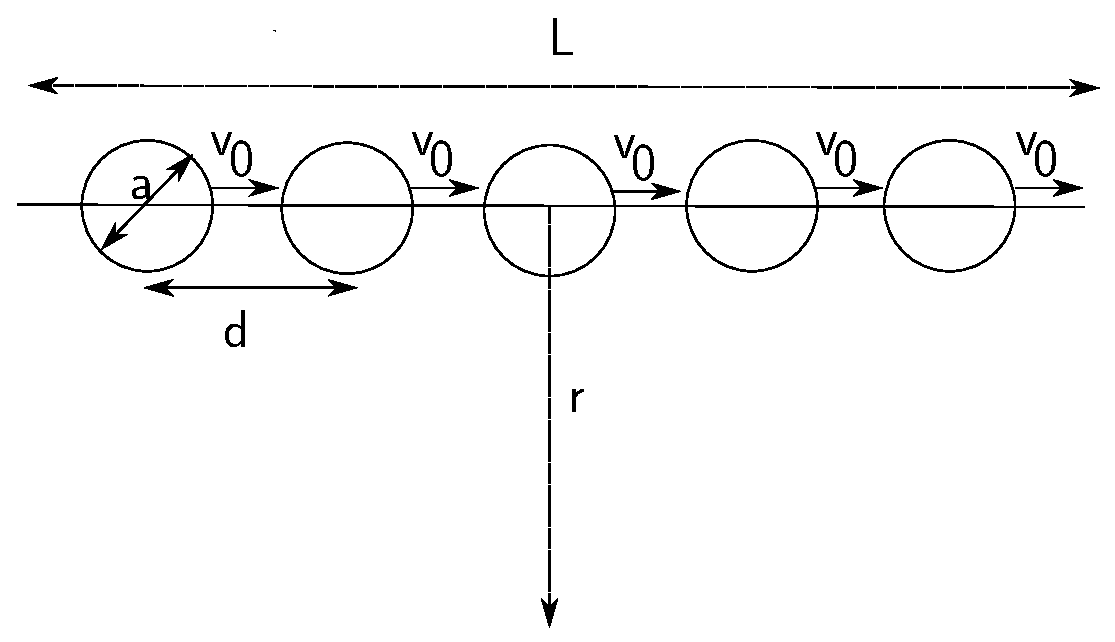
\includegraphics[width=\hsize]{spheres.eps}
\caption{ 
A train of spherically shaped impellers of diameter $a$ and separation $d$, all moving in a fluid with a velocity $v_0$.
The velocity is measured at a point a distance $r$ from the axis.
}
\label{fig:spheres}
\end{center}
\end{figure}

\section{Enhancement of Streaming Due to Hydrodynamics} 

Consider impellers to be objects each with maximum linear dimension
$a$, and with a mean spacing of $d$ arranged in a straight line as shown in Fig ~\ref{fig:spheres}. 
These impellers are pictured as spheres, but hydrodynamics is not sensitive to
the exact shape of an impeller, as it depends mainly on its maximum linear dimension~\cite{BergRandomWalksinBiology}. 
We will
now analyze the amount of streaming due to motion of these impellers
moving on a single microtubule. We initially consider the impellers to be much larger than
the kinesin molecules so that they dominate the hydrodynamical response
of the fluid.

If spherical impellers were close-packed along the microtubule, that is $a \approx
d$, then this problem would be equivalent to a single rod of length $L$
moving at constant velocity $v_0$ in the fluid in a direction parallel
to its long axis.  In that case, the velocity field for distances
$r \ll L$ has only a weak logarithmic dependence of $r$, meaning that up
to a correction of order $\ln(L/a)$, the velocity field is only weakly
dependent on distance and of order $v_0$. (Here we take the velocity of the fluid
to go to zero far from the rod.)
This is related to the well
known result that the drag on a rod of length $L$ is of the same order
as that of a sphere of diameter $L$ despite the latter's much greater volume~\cite{BergRandomWalksinBiology}. Such a system of densely packed impellers would
be very efficient at driving fluid motion and only a low density of microtubules
would be needed for cytoplasmic streaming.

Now consider the more realistic case in which the impeller size is less than
the spacing between them, which is much less than the length of a
microtubule, that is $a < d \ll L$.  At a distance $r \gg d$, the
velocity field will behave just as in the closed-packed case except appear
to have a diminished impeller velocity. That is for $d \ll r \ll L$,
the magnitude of the velocity $v(r)  = v_0 f(a/d) g(r)$, where $g(r)$
contains all the distance dependence of the velocity field, and $f(a/d)$
is how the velocity scales with the ratio of $a/d$. In the limit where
$a/d$ is very small, the system becomes dilute and the velocity between 
impellers will decay to zero. We recover the motion of isolated impellers
in this case, where it is well known (e.g. Stokes' drag) that the velocity
field is proportional to $a$. Therefore for small argument $x$, $f(x)$ is
linear (in other words, the fluid velocity is proportional to $a$.) 

Using this general argument we conclude that, independent of the exact shape of the impellers,
the flow velocity is reduced from the closed-packed case by a factor $\sim a/d$. The effect
of the impellers only starts decreasing substantially at a distance of order the
length of the microtubule $L$, below which it should only have a weak logarithmic
dependence. In other words, for a spherical region just enveloping a microtubule,
the fluid velocity is slowly varying and reduced from the kinesin motor velocity 
by a factor of order $a/d$.


Of course there are  many microtubules in these cells. To understand how this
affects the above analysis, consider all space filled with an infinite forest of them all oriented
in the same direction. 
First if we ignore the microtubules and just consider the spherical impellers, then
if we move to a reference frame moving with the impeller velocity, the system is static
and the velocity everywhere is zero. Therefore in the original reference frame, the
fluid is also moving uniformly at the impeller velocity. This is not correct because
we have ignored the hydrodynamic drag of the microtubules represented by the line going through
the spheres in Fig. \ref{fig:spheres}. To estimate their effect on the fluid velocity, 
denote the drag coefficient on an impeller by $b_I$ and that of a section of microtubule length $d$ by $b_M$. Then
we go to a reference frame velocity $v$ such that the total force acting on the combined system of
impellers and microtubules is zero, so that $b_I(v_0 - v) - b_M v = 0$, or $v = b_I v_0/(b_I + b_M)$.
Because the net force acting on this system is zero in this frame, $v$ is the velocity
of the fluid far from the microtubules.
Because within logarithmic corrections, the drag coefficients are proportional to the maximal
linear dimensions, then a conservative estimate of
this speed is of order $v_0 a/d$. The exact formula depends on the shape of
the impellers. This argument assumes an infinite volume of
microtubules but the corrections to this due to the finite nature of the system
are not important for the estimates we are making.

The identities of impellers in this system are still unknown but there are many possible
candidates. Anything with  large linear dimensions in at least one direction 
will give a large hydrodynamic radius $a$~\cite{BergRandomWalksinBiology}. The
other requirement is that it can attach to kinesin.  In fact
it is possible that the impellers in this situation could themselves be microtubules that are
not attached to the cortex~\cite{WangRiechmann,Seeger}.
Experimental estimates of the cytoplasmic streaming velocity
are approximately $0.25 \mu m/s$, about $\frac{1}{4}$ to $\frac{1}{2}$ the typical velocity of a kinesin
molecule. This suggests that $a/d$ is $\frac{1}{4}$ or greater.
For example, if we take the maximum dimensions of an impeller to be $250 nm$,
this predicts a spacing between impellers of $1 \mu m$ or less.

Another important biological issue is the necessity to have some microtubules in direct physical contact
with the cortex of the
oocyte, for example by tethering or by frictional forces. A free floating microtubule with kinesin moving on it will apply {\em zero} net force
to the fluid. This is a simple consequence of Newton's third law, or equivalently, conservation
of momentum. This does not contradict
the fact that bacteria are able to swim: the force propelling the bacterium forward is
countered by an equal and opposite force on the environment, leading to velocity fields that
are dipolar at large distances. Unlike the case analyzed above, this will not lead to long range hydrodynamic motion
of the fluid and will not lead to efficient cytoplasmic streaming by relatively few motor proteins. 
Contact with the cortex is crucial as it allows for transfer of force from outside of
the oocyte to the cytoplasm enabling fast streaming of the bulk to be powered by a much smaller volume of kinesin driven
impellers.

\section{Travelling Wave Instability of Microtubules}

We now show how the kinesin generated tangential forces on microtubules give rise to travelling wave conformations 
and calculate their angular and spatial frequency.
A microtubule has a configuration $\br(s)$ parameterized by 
an arclength $s$ and, at long enough length scales, can be modeled as being inextensible, 
that is $|\partial \br/\partial s| = 1$
with an elastic bending constant $C$. The inextensibility is enforced by a position dependent tension $T(s)$. 
There is also a force acting on the microtubule as a result of kinesin walking along it.
The magnitude of the force is proportional to the local speed and the size of the kinesin-driven impeller
and the direction of the force is tangent to the microtubule,
which, we will see, has the effect of making it buckle. We denote this with a force per unit length of $f_k$. 
We also include a force due to the cytoplasm streaming at a velocity $v_s$ which
we take to be in the $\hat k$ direction away from the minus end and this force tends to straighten the microtubule. This leads to the equation
\begin{equation}
\label{eq:microtubule}
\nu \frac{\partial \br}{\partial t} =  -C \frac{\partial^4 \br}{\partial s^4} + \frac{\partial}{\partial s}(T(s)\frac{\partial \br}{\partial s}) -
f_k \frac{\partial \br}{\partial s} + \nu v_{s}{\hat k} .
\end{equation}
where $\nu$ is a hydrodynamic drag coefficient per unit length. 

\begin{figure}[htp]
\begin{center}
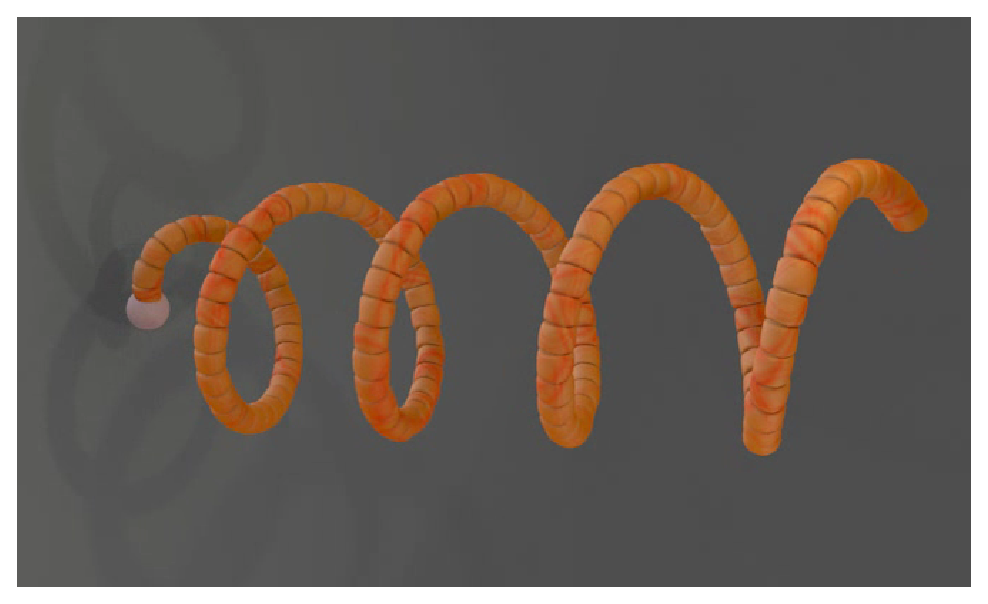
\includegraphics[width=\hsize]{simulation1.eps}
\caption{ 
The motion of a microtubule with a constant force being applied tangent to its axis. 
A constant velocity in the horizontal direction  from left to right has also been applied representing
the background from cytoplasmic streaming. The white ball on the left represents
the point at which the microtubule's minus end is tethered. See supplemental
movie 1~\cite{SupplMovies}. In a real oocyte, the radius of curvature would
correspond to approximately $40 \mu m$ and the dimensions of the entire figure are
roughly comparable to the oocyte. The thickness of the microtubule has been magnified
by a factor of about $2000$ to facilitate viewing.
}
\label{fig:simulation}
\end{center}
\end{figure}


We first implemented this equation numerically for a range of parameters
and enforced boundary conditions that tethered the minus end against the cortex, while
the plus end was free. Starting from random initial conditions, the equation rapidly goes to a steady state that
typically is described by a curve that asymptotically becomes helical for large $s$ and rotates uniformly at constant
angular velocity. The results of a steady state configuration are shown in Fig. \ref{fig:simulation}. 
The supplemental movies~\cite{SupplMovies} discussed below, show microtubule solutions for different
parameters.
Supplemental movie 1 shows the full time dependence~\cite{SupplMovies}. The chirality of the helix depends on its initial conditions.
Therefore the direction of rotation is random but stable once steady state is reached.

As the microtubule is made longer, the angular velocity and radius of the helix go to
a constant limit. However the tethered part is not helical but nevertheless rotates
in synchrony with the rest of the microtubule. These dynamics we analyzed in detail
(see the supplemental information) to find the form of the solution to this equation.
In particular we show that this equation supports travelling waves and find the
relationship between the angular velocity of rotation $\omega$ and the asymptotic
radius of the helix, and the external velocity fields $v_s$. In the case where $v_s = 0$, the
relationship simplifies to 
\begin{equation}
\label{eq:Romega}
\nu R \omega/f_k = 1.
\end{equation}
independent of chain length.

It is interesting to note that for travelling waves, solutions can be at any scale. There is a continuous family of solutions
all with the same shape but different scale factors. In the case of a helix, many different radii $R$ are solutions to
these equations.

What determines the value of $R$ that is selected? As with other problems in pattern formation such as the ``geometric model"~\cite{Kessler}
or the full dendrite problem~\cite{Barbieri}, it is the boundary conditions
that are responsible for the unique value of $R$ that is selected. In this case, the microtubule minus end is tethered, $\bu(0) = 0$
but the plus end is free.
The solution will only exist for discrete values
of $\beta \equiv C/(R^3 f_k)$. Numerical analysis gives, $\beta = 0.05 \pm 0.0005$. 
This implies that 
\begin{equation}
\label{eq:R}
R =  (C/(\beta f_k))^{1/3}.
\end{equation}

This analysis was extended to non-zero $v_s$ and as shown in the supplemental materials~\cite{SupplMat}, does not
appreciably change the estimate we will give below for microtubule wave parameters in fast streaming oocytes. 


When the microtubule is tethered to an impenetrable surface (in this case, the oocyte cortex) and the external cytoplasmic streaming velocity $v_s$
is parallel to that surface, the form of the solution changes considerably. Numerical results show that the microtubule becomes completely two dimensional,
lying close to the surface. For low enough $v_s$, travelling wave
solutions are close to prolate cycloids, meaning that the microtubule periodically loops back
on itself (see supplemental movie 2~\cite{SupplMovies}. This can be understood analytically. For sufficiently large $v_s$ it transitions to other states finally becoming 
two dimensional and looking close to a sinusoid (see supplemental movie 3~\cite{SupplMovies}. This is analyzed in detail in
the supplemental materials~\cite{SupplMat}.

We have not included hydrodynamic and steric interactions between
different microtubules except in the approximate way of giving rise to
a constant cytoplasmic streaming velocity. Given the microtubule density in the
oocyte, we expect these interactions to be substantial. However the wave
like motion that we find is quite robust. Attaching microtubules together or
considering additional forces still leads to periodic or sometimes chaotic
motion, still at the same characteristic time and spatial scales. Therefore
despite the simplicity of the model, we expect that the basic length
and time scales that we predict should be quite robust.

\section{Comparison with Experiment and Discussion}

We now check to see whether the above model is consistent with experimental
results.  

Estimates of the microtubule elastic constant $C$ vary
considerably~\cite{Felgner,GittesRigidity}  but range mostly within 
$2$ to $4 \times 10^{-23} N m^2$. We estimate the force due to the kinesin
per unit length, $f_k$ to be its velocity $v_k$ times the cytoplasmic
viscosity. We will assume as suggested by our above analysis, that
$a/d$ is between $1/4$ and $1$. We will take the kinesin velocity $v_k$ to be approximately $1
\mu m/s$~\cite{SvobodaBlock,MeyhoferHoward}. The effective viscosity of the cytoplasm for small
particles has been studied extensively and appears to vary depending on the type of cell on the length scale~\cite{LubyPhelps}. 
Particles of different sizes diffusing in the cytoplasm diffuse as if the medium had a different viscosity. Its viscoelastic properties will depend on many
factors such as the state of gelation of actin filaments~\cite{YinStossel}.
We will assume that during fast cytoplasmic streaming, the cytoplasmic actin is mainly in a "sol" state allowing fast streaming
to more readily take place. If this is not the case, the effective viscosity could be much higher~\cite{LubyPhelps}
but the dissipation would increase proportionally requiring a higher energy input. 
For small particles of radius approximately $20 nm$, the effective  viscosity 
as measured by diffusion is approximately 8 times that of water~\cite{LubyPhelps} and we will use this
value for comparison with experiment.  
This gives $f_k = (a/d) v \eta$ in the range  $2$ to $8 \times 10^{-9} N/m$.
Plugging these numbers into Eq. \ref{eq:R} gives $R$ in the range  $30$ to $50 \mu m$.
We can estimate the angular velocity using Eq. \ref{eq:Romega} (which
ignores cytoplasmic streaming). To get the largest range of times, we assume that the hydrodynamic drag
coefficient is due solely to the impellers, so that $\nu = (a/d) \eta$. This
is equivalent to $\omega = v_k/R$ or a period of $ T = 2 \pi R/v_k$ which ranges 
from $190$ to $310 s$.

Serbus and colleagues have observed microtubule behavior in living Drosophila oocytes using GFP-tubulin 
and confocal fluorescence microscopy~\cite{SerbusSaxton}. 
Time-lapse movies showed bright fibrous fluorescence, representing
groups of microtubules, in a background of diffuse fluorescence from non-polymerized GFP-tubulin.
The microtubule patterns changed over time, as did the patterns of motion of organelles that
either excluded the GFP-tubulin or were themselves auto-fluorescent. Bends in the microtubules were
at times visible in the $x-y$ optical plane and some remained visible within that plane for $30-90 s$,
allowing measurement of a radius of curvature that we expect to approximately correspond to the
$R$ in the above analysis. $R$ was measured  to be $19.5\pm 6.5 \mu m$ with $9$ measurements (standard error $2.1 \mu m$),  and
the wave velocity was $v = 0.265 \pm 0.04 \mu m/s$ with $4$ measurements. Because these waves
appear roughly sinusoidal, we can also estimate the period $T$. Assuming a wavelength of $4R$
then the measured velocity gives a period of $T= 294 s$ with an even larger error bar
considering the fact that this assumes a waveform that is probably not accurate. Nevertheless
it suggests a characteristic time.



The motion studied here can be contrasted with ciliary
motion~\cite{Kennedy} which has a period on the order of $.05 s$. Clearly
the two mechanisms have fundamentally different explanations. 
The experimental time scale points to the mechanism described here rather
than ciliary motion.  The agreement found with experiment in our above
analysis is to some extent fortuitous, given the large uncertainties
in the experimental system. But nevertheless, it provides evidence that
the simple mechanism proposed is the origin of the behavior seen in
cytoplasmic streaming.  The experimental evidence~\cite{SerbusSaxton} that dynein inhibits
streaming and that minus ends of microtubules are in contact with the
cortex~\cite{ChaSerbus}, both support this hypothesis as well. 

More generally, the above analysis elucidates, at a qualitative level, the phenomena seen
in experiment~\cite{SerbusSaxton}, of strong cytoplasmic streaming
occurring concomitantly with wave-like motion of microtubules.
The movement of a relatively few number of kinesin motors on a microtubule 
couples to the fluid causing a bulk hydrodynamic flow. The force a
kinesin exerts on a microtubule sets the microtubule into motion causing
it to execute wave-like motion. This in turn causes the flow lines around microtubules to be time dependent,
making the microtubules act as stirrers for the surrounding fluid, which leads to 
chaotic flows and strong mixing~\cite{Aref,Aref2000}. 



\begin{figure}[htp]
\begin{center}
(a) 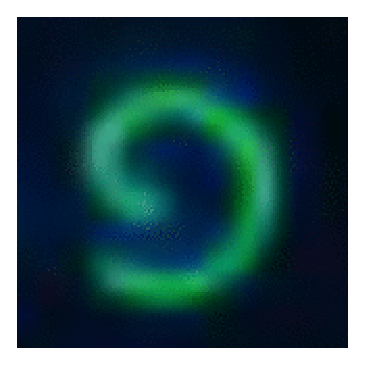
\includegraphics[width=0.3\hsize]{koch2.eps}
(b)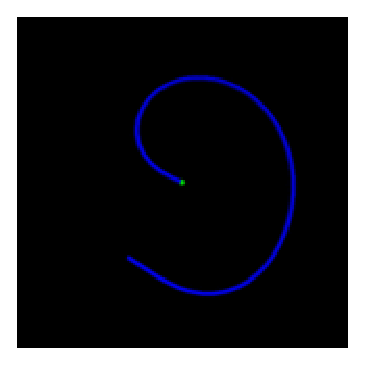
\includegraphics[width=0.3\hsize]{squiggle_sim.eps}
\caption{ 
The configuration a rotating microtubule in a gliding assay~\cite{MaloneyHerskowitzKoch,MaloneyKochVideo} with the leading end
stuck to a kinesin protein is shown in (a). (b) Shows the two dimensional simulation
of Eq. \ref{eq:microtubule} showing a similar shape.
}
\label{fig:squiggle}
\end{center}
\end{figure}


Can such motion be directly observed in an {\em in vitro}
experiment?  In fact it has been seen frequently as an unwanted artifact
of sample preparation.
Microtubule gliding assays were pioneered more than two
decades ago~\cite{ValeSchnappEtAl} and have become a
standard technique to better understand the motion of kinesin motors.
When a solution microtubules and ATP is placed on a glass surface on
which there is a high density of kinesin molecules, the kinesins propel
the microtubules with their minus ends leading.  Occasionally the minus
end sticks, perhaps to damaged kinesins, and continued forces of the
trailing portion of the microtubule cause flexing and curve generation.

Microtubule gliding assay videos of high quality~\cite{MaloneyHerskowitzKoch} provide an excellent
source of data for investigating the two dimensional version of the problem
studied here~\cite{MaloneyKochVideo}. The microtubule is being pushed by kinesin molecules
that on average, apply a force tangent to the microtubule. When an
end is tethered by sticking to a kinesin molecule, as noted above, this leads to 
a physical situation that is well described by Eq. \ref{eq:microtubule}. It should be
emphasized that the values of the tangential force $f_k$ and the drag
coefficient $\nu$ will be much larger than in the oocyte case.
Consequently, sometimes microtubules flex,, 
forming a G-shaped curve that rotates around the anchored minus end 
of the microtubule.  Fig. \ref{fig:squiggle} shows a comparison of
snapshots of the microtubule with that of a
simulation of Eq. \ref{eq:microtubule}. The resemblance is quite striking and provides evidence that
the theoretical modelling of this bending instability is valid. Note that
the shape obtained is independent of the values of model parameters. From
measuring the radius $R$ of the G-like configuration and its angular
velocity of rotation, we can compute both $f_k$ and $\nu$ from Eqs.
\ref{eq:R} and \ref{eq:Romega}, giving  $\nu = \omega C/(\beta R^4)$
and $f_k = \nu R \omega$. Measurements give $R \approx 1.33 \pm 0.2
\mu m$ and the period $T = 12 \pm 1 s$. Therefore $\nu = 133 N s/m^2$
and $f_k =  9.3\times 10^{-5} N/m$, both estimates are accurate within
a factor of 2 assuming that $C$ has been well determined.  The force
exerted by a kinesin motor in this situation is close to the experimentally determined stall
value of approximately $f_m = 5 pN$~\cite{MeyhoferHoward}. Assuming that
each motor attached can exert this force, this gives
an average distance between motors of $f_m/f_k = 53 nm$. This assumes that
the attachment of the motors is flexible enough to allow microtubule interactions capable of exerting this stall force. If
this is not the case, we expect the kinesins to be spaced more closely but
by no more than half this amount. This distance
seems reasonable given the high density of kinesin molecules attached
to the glass, and the size of the $\alpha-\beta$ tubulin dimer which is
approximately $8 nm$ in length. Thus the above considerations can give
a quantitative measure of the forces and drag in these gliding assays.


Nevertheless, it would also be of interest to verify the travelling wave solutions experimentally
in three dimensions for isolated
microtubules and kinesin, for example, by utilizing a single molecule optical trap, or by some other
means, allowing for a more rigorous test of the predictions made here.


It is of interest to speculate on the reason for this microscopic mixing
mechanism.  If the microtubules were attached from the {\em plus} end,
there would be no dynamical instability from kinesin generated forces
but the cytoplasmic streaming would be more efficient, with greater transfer
of force from outside the oocyte, because the tension at the
tether point would increase linearly with the length of the microtubule,
whereas the tension saturates to a constant value in the case considered
above. However as discussed earlier, complex stirring patterns are
expected to be far more efficacious in mixing than steady-state flows.
This agitation could then serve an important biological function.


In summary, we have found a very simple set of conditions for generating efficient mixing
in large eukaryotic cells. If microtubules are aligned so that their minus ends
are in contact with the cell perimeter and dynein is suppressed, this will lead 
(a) to cytoplasmic streaming in the bulk of the cell and (b) wave-like motion of
microtubules. The latter will promote efficient mixing of the cell's contents by
inducing chaotic flows.
The efficiency of the cytoplasmic streaming is due to the long range nature of
hydrodynamic coupling and the indirect linkage of microtubules to the oocyte surroundings via the cortex, leading to momentum transfer.
The wave-like motion is due to an instability in the dynamics which breaks chiral
symmetry and is a consequence of the tangential forces exerted by motor proteins on the elastic
microtubules. Given the uncertainties in the experimental system and approximations
made in the analysis, The wave-like motion seen in experiments agrees well with our theoretical predictions
suggesting these effects represent a robust phenomenon.
We are now engaged in experimentation to gather more accurate data on microtubule behavior 
{\em in vivo} and {\em in vitro} under various conditions in order to further understand
the mechanisms for fast cytoplasmic streaming discussed here.

The authors would like to thank Ian Carbone, and Bill Sullivan for useful discussions.
We also would like to gratefully acknowledge Andy Maloney and Steven J. Koch for their permission
to use a snapshot of their video, Fig.  \ref{fig:squiggle}(a) \cite{MaloneyKochVideo} of their
experimental results~\cite{MaloneyHerskowitzKoch}. This was generously distributed to us
by them~\cite{KochLab} through the practice of Open Notebook Science~\cite{OpenNotebookScience} 
This material is based upon work supported by National Institutes of Health GM046295 (to W.M.S.), National Science Foundation
CCLI Grant DUE-0942207 (to J.M.D.),
the  Defense Threat Reduction Agency basic research grant HDTRA-1-09-1-0018 (to Steven J. Koch),
and the National Science Foundation IGERT Grant DGE-0549500 (to Steven J. Koch).



%Single chain math Paper
\section{Motion of Microtubule With Kinesin Walkers}

Here we study the motion of microtubules in the context of cytoplasmic
streaming in stage 10B-11 Drosophila oocytes.  At that stage, the roughly
hemispherical oocyte is bounded by a plasma membrane and an underlying
cortex comprised of an actin filament meshwork.  Long microtubules,
with minus ends attached to the cortex, have their plus ends free.
Kinesin-1 motor proteins that walk along the microtubules toward plus
ends generate opposing forces on the microtubule and the surrounding
viscous cytoplasm.  Cytoplasm is thus moved toward plus ends, generating
vigorous flows for mixing.  Because minus ends are anchored, the equal
but opposite force on a microtubule generates dynamic bending along
its length.  The results of this work have been used to understand this
phenomenon in recent work by the authors~\cite{DeutschBrunnerSaxton}.

We begin with the equation for a microtubule with an applied force tangent to the direction of chain. The position
of the microtubule at arclength $s$ and at time $t$ is denoted $\br(s,t)$. As is usual at small scales, all inertial effects are negligible
and the system is dominated by the drag coefficient per unit length $\nu$,
\begin{equation}
\label{eq:microtubule}
\nu \frac{\partial \br}{\partial t} =  -C \frac{\partial^4 \br}{\partial s^4} + \frac{\partial}{\partial s}(T(s)\frac{\partial \br}{\partial s}) -
f_k \frac{\partial \br}{\partial s} + \nu v_{s}{\hat k} .
\end{equation}
$C$ denotes the elastic bending constant of the microtubule. The tension $T(s)$ enforces the inextensibility of microtubules which
can be written as  $|\partial \br/\partial s| = 1.$ 
Kinesin motors walking along the microtubule are assumed to be carrying cargo that acts as an impeller pushing the surrounding
cytoplasmic medium. By Newton's third law, this force produces a drag on the impellers that transmits this force to the
attached microtubule. Assuming a high density of kinesin walkers, the effective force on the microtubule will be in the
direction of the local tangent to $\br(s)$ which is $\partial \br/\partial s$. The coefficient $f_k$ gives the strength of the force.
Lastly we add a uniform flow field representing the velocity of the cytoplasm $v_s$ in the vicinity of the microtubule
which we take to be in the $\hat k$ direction.

We rescale to dimensionless variables 
\begin{equation}
\label{eq:rescale}
\sigma = s/\rho_0,~ \bu = \br/\rho_0, ~ \tau = t \omega_0,  ~ T' = T \rho_0^2/C, ~{\rm and} ~ h = \nu v_s/f_k 
\end{equation}
so that
\begin{equation}
\label{eq:dimensionless}
\frac{\partial \bu}{\partial \tau} =  - \frac{\partial^4 \bu}{\partial \sigma^4} + \frac{\partial}{\partial \sigma}(T'(\sigma)\frac{\partial \bu}{\partial \sigma}) -
\frac{\partial \bu}{\partial s} + h {\hat k} .
\end{equation}
This requires that 
\begin{equation}
\label{eq:scaling}
\omega_0 = f_k/(\nu \rho_0), ~  {\rm and} ~ \rho_0^3 = C/f_k. 
\end{equation}
$\rho_0$ and $\omega_0$ are constants that make our new variables dimensionless.

We will consider solutions where one end (the {\em minus} end) is tethered to a point, say the origin, so that
$\br(s=0,t) = 0$ and is freely hinged at that point. The other end is free.
The total arclength of the microtubule is denoted by $L$.
The general characteristic of all numerical solutions to Eq. \ref{eq:microtubule} is that
for large $s$ the solutions appear to be travelling waves. In fact, the form of solution
becomes independent of $L$ so in fact we could consider this problem in the limit $L\rightarrow \infty$.
For example we find solutions that asymptotically become helical with a fixed path and radius for
large $s$. Other solutions are planar and are periodic in $s$. In all these cases the solution
has the form of a travelling wave that we analyze in detail below.

\section{Steady State Travelling Wave Solutions}

Now we look for steady state travelling wave solutions. First we clarify what this means.
The whole microtubule should not be translating because one end, (far away from where
the travelling wave solution is valid) is tethered. 
The position averaged over one period of a monomer, $\langle u \rangle$, should be  time independent.
If the microtubule is stretched out
in one particular direction, there should be a displacement $\bu_d$ of the microtubule about a straight
line solution,
\begin{equation}
\label{eq:travelling}
\bu(\sigma, \tau) = \bu_d(\sigma-v\tau) + \alpha \sigma {\hat k}.
\end{equation}
The term $\bu_d$ describes a displacement that travels along the backbone of the chain maintaining its shape.
Therefore we require
\begin{equation}
\label{eq:ud_constraint}
\frac{\partial \langle \bu_d \rangle}{\partial \sigma} = 0
\end{equation}

Substituting Eq. \ref{eq:travelling} into Eq. \ref{eq:dimensionless} gives a left hand side
of $-v \partial \bu_d/\partial \sigma$ and a term of the form $-\partial \bu_d/\partial \sigma$ on
the right hand side. Choosing $v = 1$ and in addition $\alpha = h$, we are left with

\begin{equation}
\label{eq:reduced_steadystate}
\frac{\partial^4 \bu}{\partial \sigma^4} + \frac{\partial}{\partial \sigma}(T'(\sigma)\frac{\partial \bu}{\partial \sigma}) = 0.
\end{equation}
We define $\bw = \partial \bu/\partial \sigma$  and
note that the inextensibility requirement $|\partial \br/\partial s| = 1$ implies that $|\bw| = 1$. We can write 
\begin{equation}
\label{eq:bw=bd_alpha}
\bw  = \frac{\partial \bu_d}{\partial \sigma} + \alpha {\hat k}
\end{equation}
Note that $\bw(\sigma,\tau)$ depends only on $\sigma -\tau$. Because $\bw$ is a function
of only one variable $\xi \equiv \sigma -\tau$, 
we can 
integrate Eq. \ref{eq:reduced_steadystate} with respect to $\xi$ obtaining
\begin{equation}
\label{eq:sphericalmotion}
\frac{d^2 \bw}{d \xi^2} - T'(\sigma)\bw = -g {\hat k}.
\end{equation}
The integration constant on the right hand side $-g {\hat k}$ must lie in the $\hat k$ direction by symmetry.
This is the same equation as that of the classical mechanics of a particle of unit mass, with position $\bw$ travelling on the surface of a 
unit sphere under the influence of gravity, with the variable $\xi$ being analogous to time. The term $-T'$ is a normal
force that constrains the particle to stay on the sphere's surface.

From Eq. \ref{eq:ud_constraint} and Eq. \ref{eq:bw=bd_alpha} we see that the motion is subject to the
constraint
\begin{equation}
\label{eq:alpha_constraint}
\langle \bw \rangle = \alpha {\hat k}
\end{equation}
The constant $g$ and the initial conditions of the particle must be chosen so as to satisfy this constraint.
There is an infinite number of solutions satisfying these conditions leading to different 
steady state solutions for the microtubule.

The spherical pendulum Eq. \ref{eq:sphericalmotion} has been analyzed~\cite{CushmanBates} in detail. In general
the orbits will not be closed, but we will relegate
our discussion below to two cases where this is the case, circular motion in Eq. \ref{eq:sphericalmotion}, corresponding to helical
conformations of a microtubule, and motion in the $x-z$ plane, corresponding to solutions similar in shape to cycloids.

\subsection{Scale Invariant Family of Solutions}
\label{subsec:ScaleInvariance}

One important point to notice about the general structure of Eq. \ref{eq:sphericalmotion} is its invariance under
change of $\xi$, that is $\xi \rightarrow \lambda \xi$. A change in scale of $\lambda$ does not modify the
solution, because $T'(\xi)$  and $g$ are both constraints, and can therefore be chosen arbitrarily. So that if
$\bw(\xi)$ is a solution to Eq. \ref{eq:sphericalmotion}, so is $\bw(\lambda \xi)$. Furthermore all solutions
of this form will have the same $\langle \bw \rangle$ and hence the same $\alpha$. Note that a length scale
shift of $\bw = \bw_0(\lambda \xi)$ corresponds to a displacement of $\bu = (1/\lambda)\bu_0(\lambda \xi)$, which
changes scale because of the $1/\lambda$ prefactor in this expression. This means that for every
steady state conformation of the microtubule, there exists a family of steady state solutions with identical
shape but arbitrary size.

\subsection{Circular Orbits}
\label{subsec:CircularOrbits}

Circular orbits are solutions to Eq. \ref{eq:sphericalmotion}. Eq. \ref{eq:alpha_constraint} requires that the vertical
height of the orbit be at $w_z = \alpha$. Therefore the radius perpendicular to $\hat k$ (the $w_x, w_y$ plane) is 
\begin{equation}
\label{eq:w_perp_alpha}
w_\perp \equiv \sqrt{1-\alpha^2}. 
\end{equation}
It is first easiest to analyze this by direct analogy to the classical mechanical problem of a unit mass particle moving on a unit sphere (the
spherical pendulum).
If the height above the sphere is $\alpha$, then application of Newton's laws gives that the tension must balance the force
of gravity $g$ and the centripetal acceleration $v^2/w_\perp$ giving
\begin{equation}
\frac{g}{v^2} \equiv \frac{\alpha}{1-\alpha^2} 
\end{equation}
Where $v$ is not the real velocity of the microtubule but $|d \bw_\perp/d\xi|$. This is the rate at which the
tangent vector rotates in the $x-y$ plane. 
Because $|d\bu_d/d\xi|  = |\bw_d| = r_c$ is a constant, $\bw_d$ is a circle. 
Therefore according to Eq. \ref{eq:travelling}, this will give a helical conformation of the microtubule. 


In the spherical pendulum analogy, the angular velocity of the particle
is $\Omega_p = v/w_\perp$. The total arclength of the chain (in dimensionless units) of a single period of
the chain is
\begin{equation}
\label{eq:SRalpha}
S = \frac{2\pi R}{\sqrt{1-\alpha^2}}
\end{equation}
and $S \Omega_p = 2 \pi$ so that $S = 2\pi/\Omega_p = w_\perp/v$. Comparing this with Eq. \ref{eq:SRalpha}
we obtain 
\begin{equation}
R = \frac{w_\perp}{v} \sqrt{1-\alpha^2}. 
\end{equation}
Using Eq. \ref{eq:w_perp_alpha} this gives 
\begin{equation}
\label{eq:Ralpha_v}
R = \frac{1-\alpha^2}{|\frac{d w_\perp}{d \xi}|} = \frac{1-\alpha^2}{v}
\end{equation}
Because $g$ is a free parameter, $v$ can be any positive number and therefore Eq. \ref{eq:Ralpha_v}
implies that the radius of the helix can be arbitrary. 

Because the velocity of this travelling wave is unity, the spatial and temporal periodicities are equal. 
Therefore the period of rotation of the helix $P'$ is equal to  $S$ in Eq. \ref{eq:SRalpha}, in the dimensionless units that we are using.
Therefore the relationship between the period and the pitch is
\begin{equation}
\label{eq:Pdimensionless}
P' = \frac{2\pi R}{\sqrt{1-\alpha^2}}
\end{equation}
In terms of our original units the period is
\begin{equation}
\label{eq:T_circle}
P = \frac{2\pi R \nu}{f_k \sqrt{1-\alpha^2}}
\end{equation}

\subsection{Two Dimensional Solutions}
\label{subsec:2dsolns}

We now consider orbits in the $x-z$ plane. This corresponds to a pendulum swinging around vertically through the bottom of the sphere.
This is a standard introductory mechanics problem. Letting $\theta$ denote the angle with respect to the $-{\hat k}$ direction,
\begin{equation}
\label{eq:pendulum}
\ddot{\theta} = -g \sin\theta 
\end{equation}
where the dots that normally represent a time derivative are really derivatives with respect to $\xi$. Low energy solutions
where the total energy $E$ is less than $g$ give $\theta$ oscillating between two bounds. 
In this case the curve for the microtubule will look sinusoidal. Beyond the separatrix where $E > g$, $\theta$ will
increase without bound. This gives rise to microtubule conformations that look close to prolate cycloids. In other words,
the microtubule forms a travelling wave that periodically loops backwards. This is shown in Fig. \ref{fig:prolate}

\begin{figure}[htp]
\begin{center}
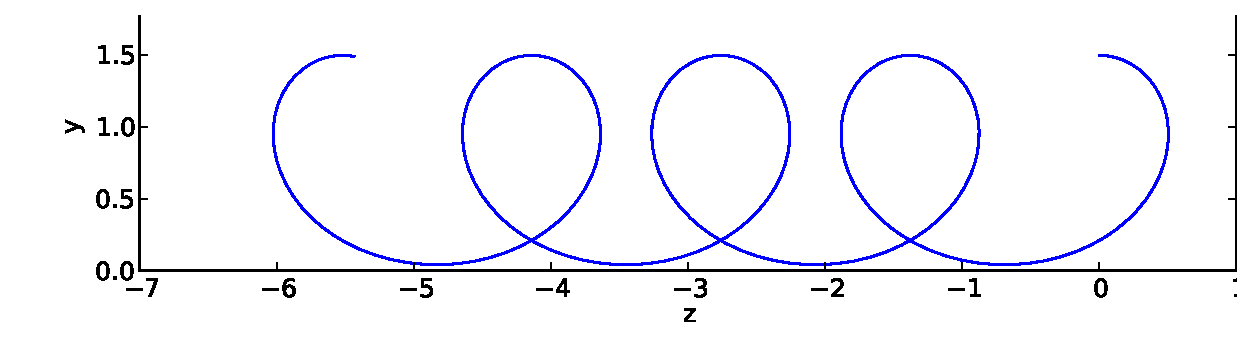
\includegraphics[width=\hsize]{shape1.eps}
\caption{ 
A two dimensional travelling wave solution for a microtubule that looks close to a prolate cycloid but
differs from it in functional form.
}
\label{fig:prolate}
\end{center}
\end{figure}

Small values of $|\alpha|$ correspond to low values of $g/E$. In this case, the particle spends almost
equal times at all points on the circle giving a small value of $\langle w\rangle = \alpha$. As $g/E$
increases to $1$, $\alpha$ increases and the loops become tighter; a situation that is very costly energetically.
However this is not the only solution to these equations for a fixed value of $\alpha$. If instead we
consider solutions with $E < g$, then large $g/E$ corresponds to small oscillations of $\bw$ about $-{\hat k}$.
In this case, $|\alpha|$ is close to $1$ and the curve has no tight loops. The shape of the microtubule
is close to a sine wave.

To obtain the relationship between $G \equiv g/E$ and $\alpha$ we use conservation of energy
to obtain the period $T$,
\begin{equation}
\label{eq:pendulumenergy}
\dot{\theta} = \sqrt{2E(1+G\cos\theta)}
\end{equation}

The time average of $\bw$ in the $\hat k$ direction is
\begin{equation}
\label{eq:avependulumcostheta}
\langle \cos\theta\rangle = \frac{\int_0^\pi \frac{\cos\theta}{\sqrt{1+G\cos\theta)}} d\theta}{\int_0^\pi \frac{1}{\sqrt{1+G\cos\theta)}} d\theta}
\end{equation}
This can be expressed in terms of elliptic integrals as
\begin{equation}
\label{eq:avecosthetaElliptic}
\langle \cos\theta\rangle =  \frac{1}{G} (1- (1+G) \frac{{\cal E}(2G/(1+G))}{{\cal K}(2G/(1+G))})
\end{equation}
Where  $\cal E$ and $\cal K$ are the complete Elliptic integrals of the first and second kind respectively.
For bounded orbits, below the separatrix, the corresponding expression can be calculated giving
\begin{equation}
\label{eq:avecosthetaEllipticBounded}
\langle \cos\theta\rangle =  -2 \frac{{\cal E}(\frac{e+1}{2})}{{\cal K} (\frac{e+1}{2}) }) + 1
\end{equation}
A plot of the $\alpha = \langle \cos\theta\rangle$ versus $1/G = E/g$ is shown in Fig. \ref{fig:AlphaVsE}
using these two expressions.
$\alpha \rightarrow 0$ in the limit as $G \rightarrow 0$. Note that there are two possible values of
$E/g$ corresponding to one value of positive $\alpha$.

\begin{figure}[htp]
\begin{center}
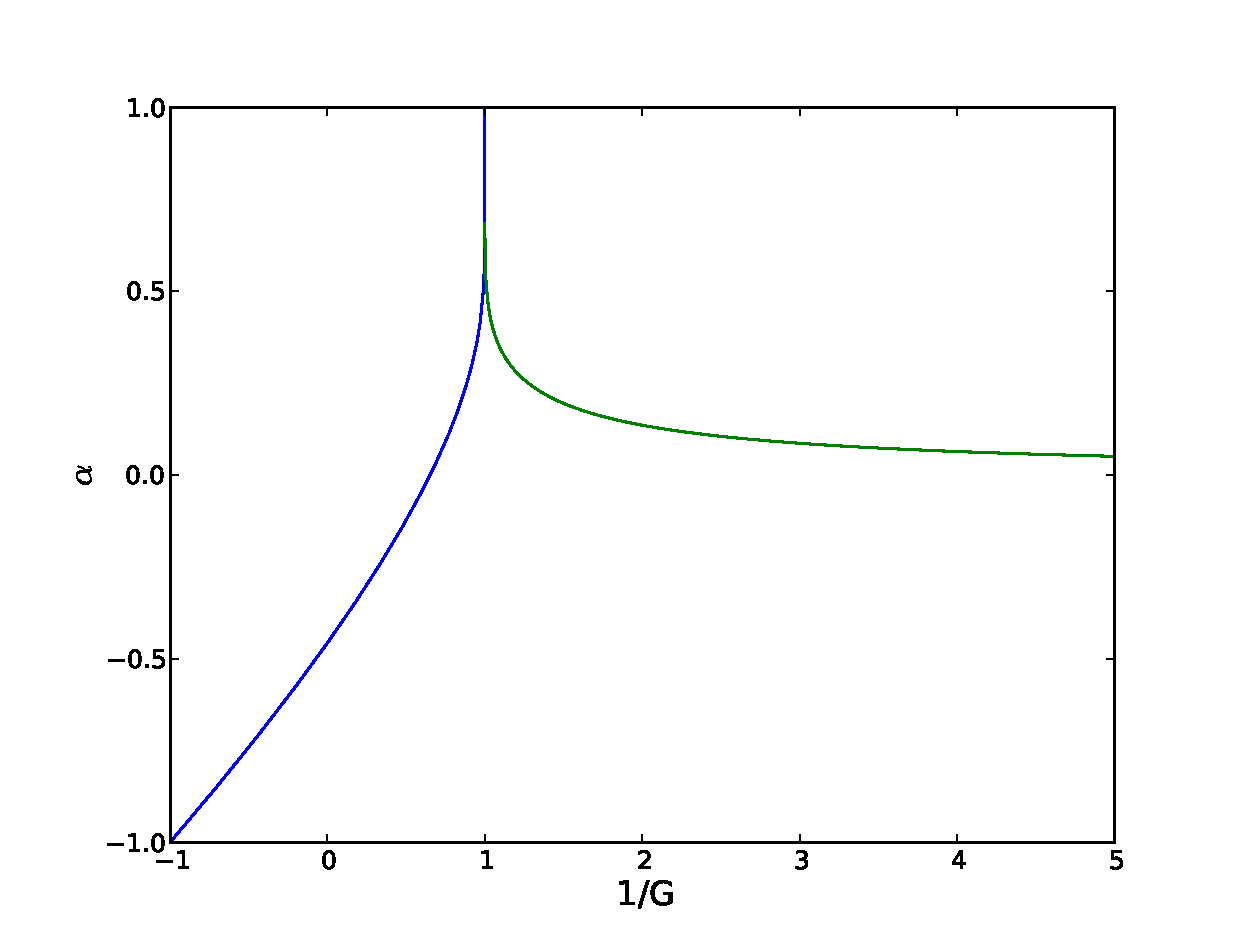
\includegraphics[width=\hsize]{alpha_vs_E.eps}
\caption{ 
A plot of the value of $\alpha$ as a function of $1/G$.
}
\label{fig:AlphaVsE}
\end{center}
\end{figure}



The case of $\alpha = 0$
corresponds to the case of circular orbits discussed in Sec.  \ref{subsec:CircularOrbits}. 
The cytoplasmic streaming velocity is $\propto h$ (see Eq.  \ref{eq:dimensionless}).
When $h = 0$, we have shown that the solutions are circular. If $h$ is now made very
small, we expect that the solution will only be slightly perturbed from circular
solutions. This corresponds to a small value of $g/E$. Therefore the value of
$G$ that is chosen for small enough $h$ should correspond to the larger value of
$1/G$ shown in Fig.  \ref{fig:AlphaVsE}. This corresponds to almost circular loops
shifting slightly forward after every turn. As $h$ increases the loops become
tighter giving rise to a high elastic bending energy. At some point therefore, 
we expect a transition to another state. In fact, simulations discussed in Sec. \ref{subsec:CompWithSims} show that near a
flat surface, the microtubule transitions out of the plane to a helical shape 
at $h \approx .385$ for $128$ links in a chain. For
still larger $h$, the microtubule becomes flat again looking close to sinusoidal.

\section{Numerical Implementation of the Full Solutions}

By comparing the steady state solutions found above for large arclength $s$ and  time $t$, we will
see that these solutions are physically realistic ones to consider. As we will see, the full
equations of motions go to solutions of this type. However this is not a complete
description of the problem, because of these solutions
a particular one is selected from a whole family of solutions. The same behavior occurs
in other problems in pattern selection such as dendritic growth~\cite{Kessler,Barbieri}.

\begin{figure}[t]
\begin{center}
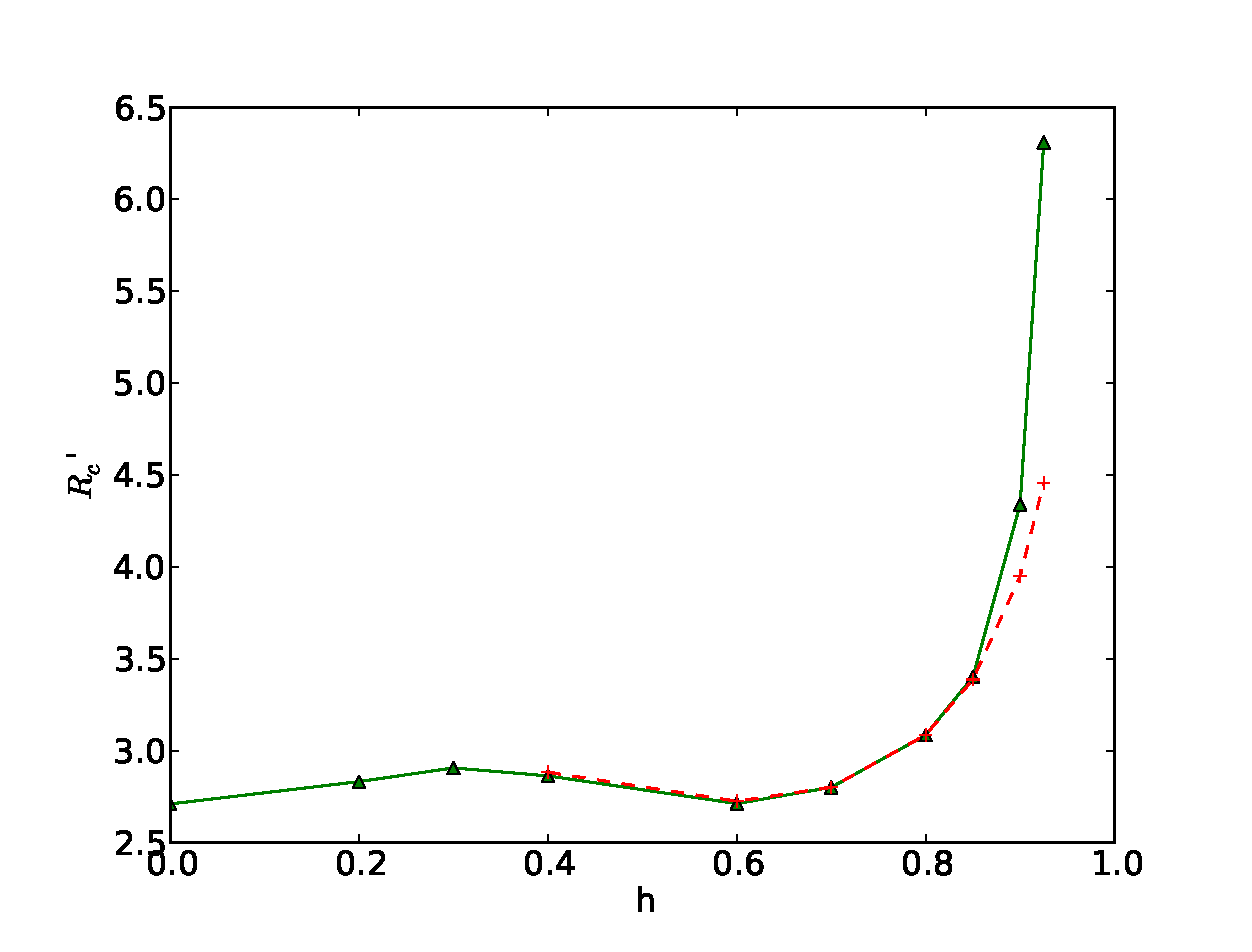
\includegraphics[width=\hsize]{rad_curv_vs_h.eps}
\caption{ 
The rescaled radius of curvature $R_c/\rho_0$ versus the rescaled velocity field $h=\alpha$.
The green triangles are for $64$ link chains, the red $+$ symbols are for chains of $128$ links.
}
\label{fig:RadCurvVSh}
\end{center}
\end{figure}

\subsection{Comparison With Simulation}
\label{subsec:CompWithSims}

Eq.  \ref{eq:microtubule} was analyzed numerically using a method similar to that
used earlier in the context of gel electrophoresis~\cite{DeutschElectrophoresisScience,DeutschMadden}.
Link length drift was handled using a similar procedure to that implemented for chains with inertia~\cite{DeutschCerfFriction}
One end was constrained to have coordinates at the origin, while the other was free. 

A Runge Kutta time step was $0.001$, $C = 20$, $f_k = 2$ and simulations were performed with $N=64$ or $N=128$ links,
as will be noted below.

We first consider the case of a microtubule with no wall or other external forces aside from the external velocity field.
As a function of the rescaled external velocity field $h$, the radius of curvature and period were calculated once the
system had reached steady state. Using rescaled variables as defined by Eqs. \ref{eq:rescale} and \ref{eq:scaling} we
can write the dimensionless radius of curvature as $R_c' = R_c/\rho_0$, and the dimensionless period as $P' = \omega P$.
The radius of curvature was calculated at the middle of the chain to reduce finite size effects.
The results are shown in Figs.  \ref{fig:RadCurvVSh} and \ref{fig:PeriodVSh}. The data for $R_c$, Fig. \ref{fig:RadCurvVSh} using
$64$ links, is very close to those of $128$ links except for the highest $h$ values. The data for the period, Fig. \ref{fig:PeriodVSh}(a)
show good agreement for both chain sizes at all values of $h$ studied.

\begin{figure}[htp]
\begin{center}
(a) 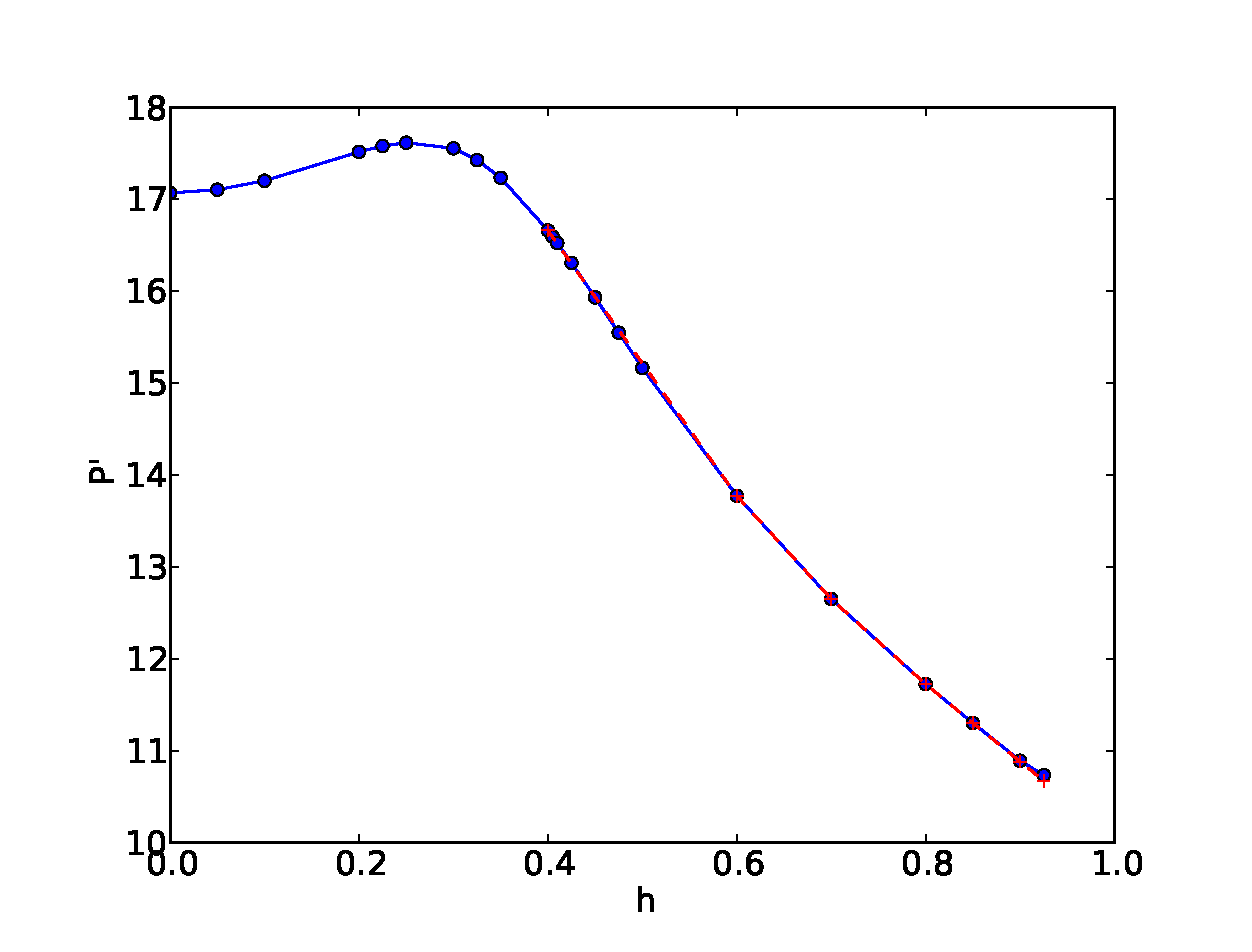
\includegraphics[width=0.45\hsize]{period_vs_h.eps}
(b) 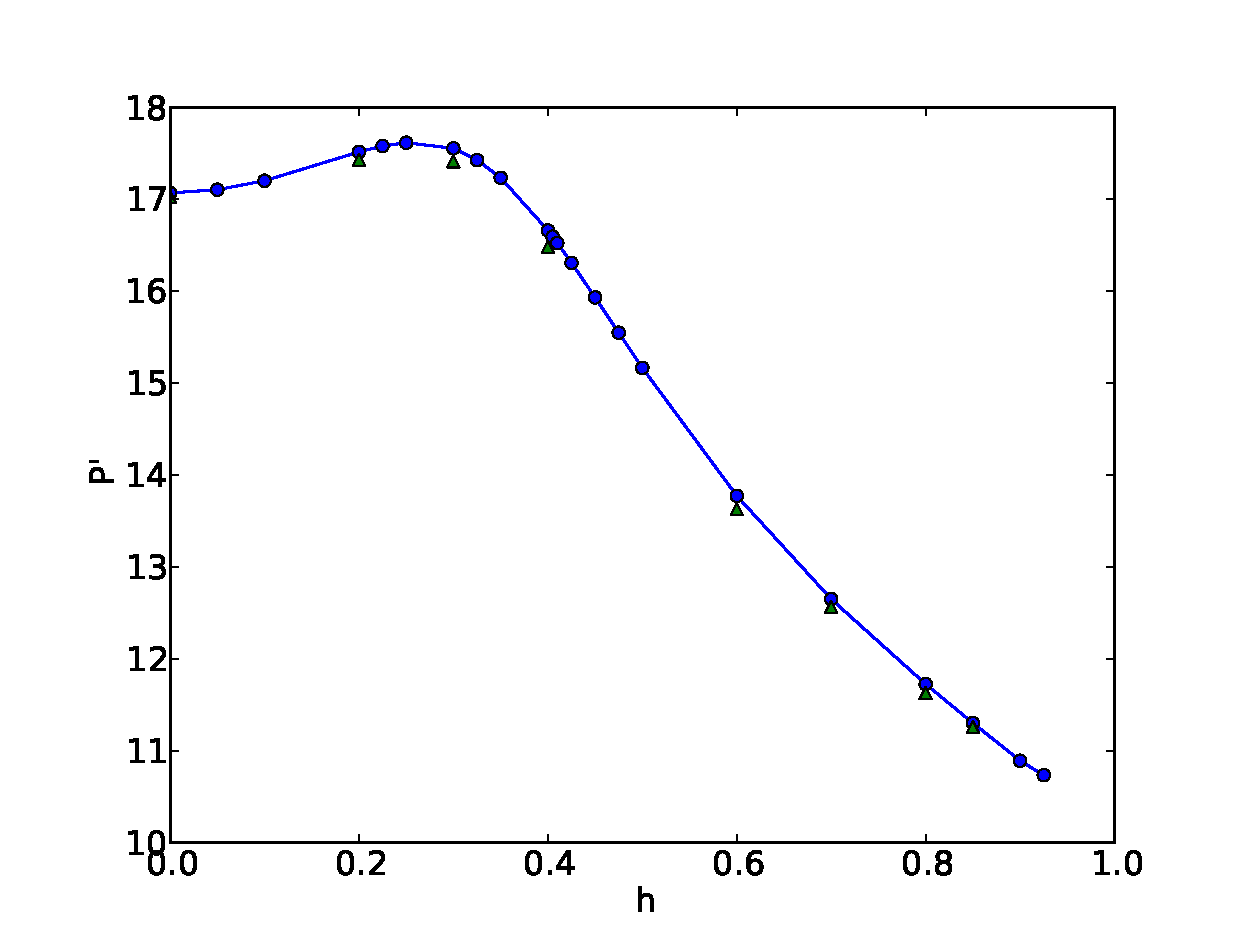
\includegraphics[width=0.45\hsize]{compare.eps}
\caption{ 
(a)The rescaled period $P' = P\omega$ versus the rescaled velocity field $h=\alpha$.
The blue circles are for $64$ link chains, the red $+$ symbols are for chains of $128$ links.
(b)
The rescaled period $P' = P\omega$ versus the rescaled velocity field $h=\alpha$
calculated by using Eq. \ref{eq:PvsRc} and data on the radius of the helix versus $h$ shown
in Fig. \ref{fig:RadCurvVSh}. The result is shown by the green triangles. 
The blue circles are the same data shown in Fig. \ref{fig:PeriodVSh} by directly
measuring the period. 
}
\label{fig:PeriodVSh}
\end{center}
\end{figure}




We now test the analytic predictions that we made relating the period to the radius of the helix and $\alpha$
given by Eq. \ref{eq:Pdimensionless}, and our conclusion that $\alpha = h$. The relationship between the
radius of curvature $R_c$ and the radius $R$ of the helix is readily calculated to be $R = R_c (1-\alpha^2)$.
Therefore Eq. \ref{eq:Pdimensionless} gives
\begin{equation}
\label{eq:PvsRc}
P' = 2 \pi R_c' \sqrt{1-\alpha^2}
\end{equation}
With this prediction and using the data for $R_c$ in Fig. \ref{fig:RadCurvVSh}, we can independently calculate $P'$ for $64$
link chains. We can only do this where finite size effects are not important and therefore omit the highest two $h$ values
from this analysis. The data, Fig. \ref{fig:PeriodVSh}(b), show excellent agreement to within the differences expected by finite size effects. This
corroborates our analytical analysis of steady state solutions. 

The case of $h = \alpha = 0$ displayed in Fig.  \ref{fig:RadCurvVSh} can be written in terms of the original
dimensional variables of Eq. \ref{eq:microtubule} using Eq.  \ref{eq:scaling}
\begin{equation}
\label{eq:R}
R_c =  (C/(\beta f_k))^{1/3}.
\end{equation}
From the numerical solution, this gives $\beta = 0.05 \pm 0.0005$. This is useful in analyzing experimental data, as
$R_c$ is nearly constant for $h < 0.7$.

Next we consider the presence of a wall. We introduced a force representing a wall in the $y-z$ plane of the form
\begin{equation}
\label{eq:wallforce}
{\bf f}_w =  \frac{x^2}{(x+1)^2} { \hat  i}  
\end{equation}
which is only present for $x < 0$. The force is singular at $x=-1$ preventing the chain from crossing that plane.
The period as a function of $h$ is shown in Fig. \ref{fig:WallPeriodVSh} for $C=20$ and chains with $128$ links.
\begin{figure}[htp]
\begin{center}
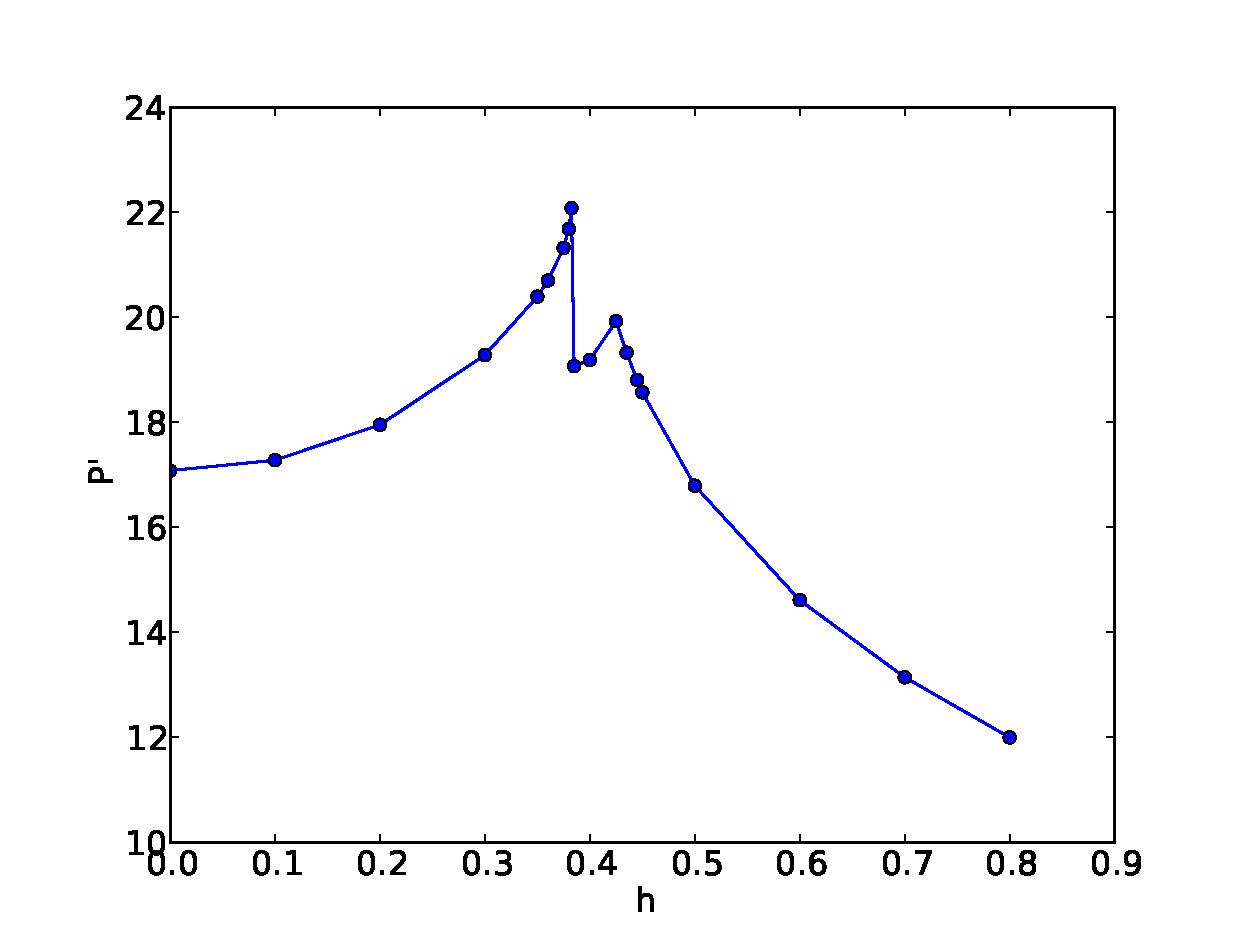
\includegraphics[width=\hsize]{wall_per_vs_h.eps}
\caption{ 
The rescaled period $P' = P\omega$ versus the rescaled velocity field $h=\alpha$
for chains of $128$ links.
}
\label{fig:WallPeriodVSh}
\end{center}
\end{figure}

For small values of $h$, the period does not vary much. The shapes obtained are flat and
appear to be the same as those found in \ref{subsec:2dsolns}. However there is non-analytic behavior at $h \approx 0.385$
corresponding to a transition to flattened helical waves. Then at $h \approx 0.425$ the solution becomes almost
completely flat and showing waves that look closer to sine waves, corresponding to the flat 
sinusoidal-like solutions studied in \ref{subsec:2dsolns}.

We now consider the dependence of period and curvature on the length of chains $L$. Our
analytical solutions have been in the limit that the chain length $L\rightarrow \infty$.
For finite length chains, we expect corrections to this behavior. This is important
to analyze in relationship to experiments using microtubule gliding assays~\cite{ValeSchnappEtAl}. In this case
we consider $h=0$ and study how the rotating spiral wave solutions vary with increasing
length. Fig. \ref{fig:RvsL}(a) shows the dependence of the radius of curvature measured
halfway along the arclength, as a function of chain length. As usual, the rescaled dimensionless
variables, see Eqs. \ref{eq:rescale} and \ref{eq:scaling} have been used. The curve
shows a non-monotonic dependence on $L$ that levels off at $L \approx 20$. 
Fig. \ref{fig:RvsL}(b) shows that the rescaled period is slightly non-monotonic as well but decreases to a constant
value at $L \approx 15$. In comparison with gliding assays, we took~\cite{DeutschBrunnerSaxton} $L = 14.0$, where
values of parameters are within $3\%$ of their asymptotic values.


\begin{figure}[htp]
\begin{center}
(a)
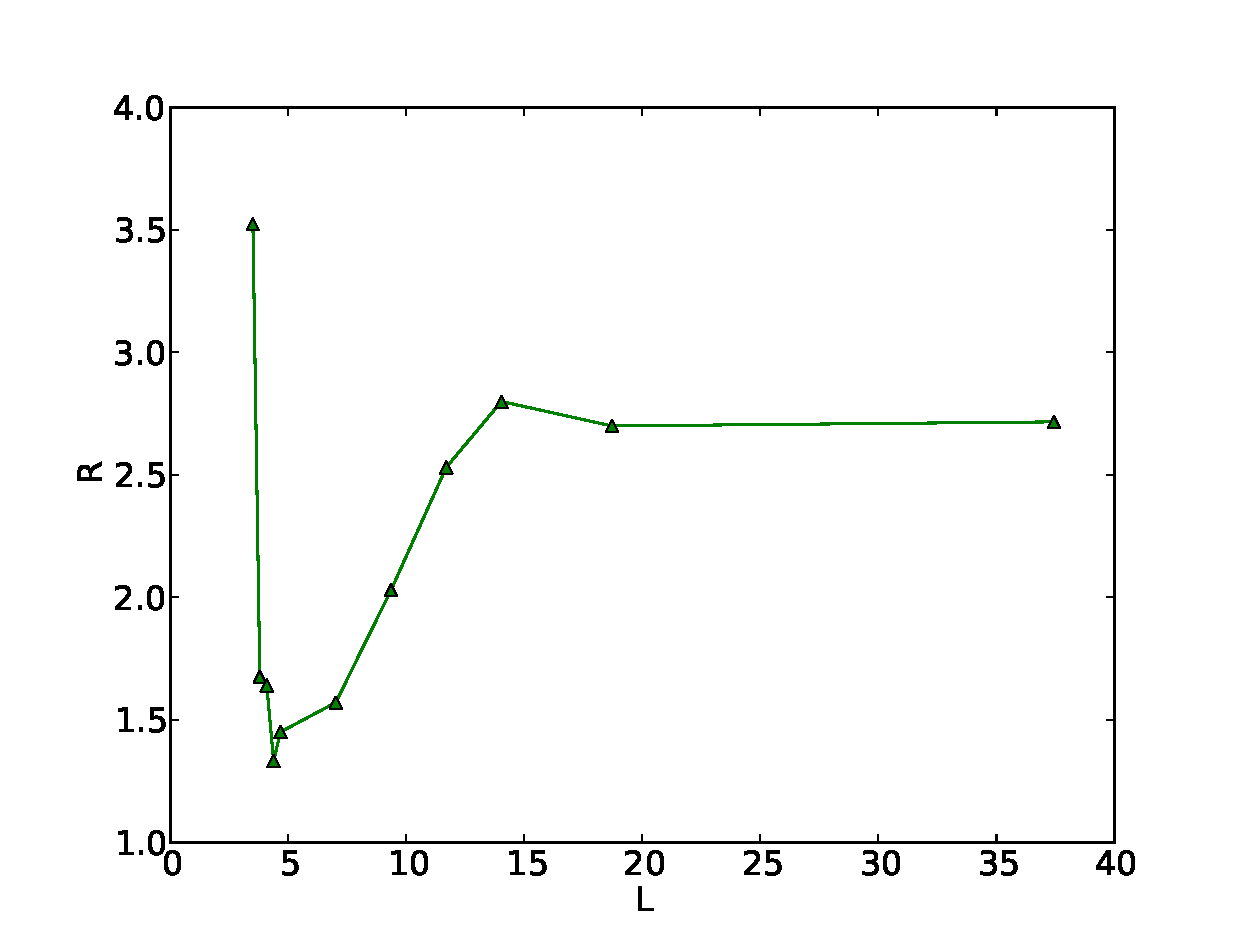
\includegraphics[width=0.45\hsize]{rc_vs_l.eps}
(b)
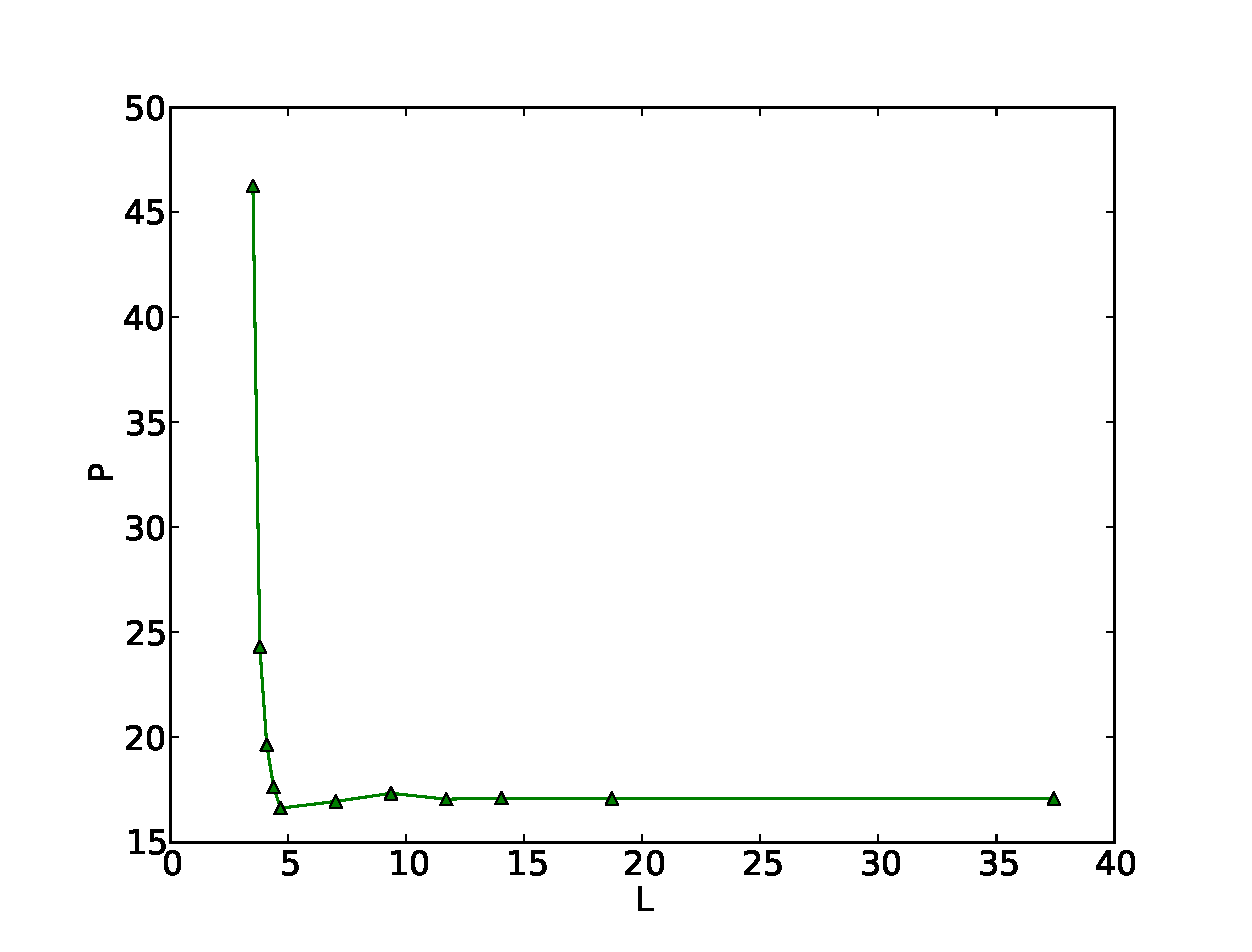
\includegraphics[width=0.45\hsize]{period_vs_l.eps}
\caption{ 
(a)
The rescaled radius of curvature measured at the middle link of a chain  versus the rescaled chain length in steady state for $h=0$.
(b)
The rescaled period  versus the rescaled chain length in steady state for $h=0$.
}
\label{fig:RvsL}
\end{center}
\end{figure}


Note that in Fig. \ref{fig:RvsL}(b) the period diverges for finite $L \approx 3$. Below this
point, the solution is a static straight line. This is similar to the usual buckling transition
for a finite length elastic rod. The microtubule needs to be sufficiently long to undergo
the dynamical instability analyzed here. 


\subsection{Selection of Scale}

As noted in section \ref{subsec:ScaleInvariance}, there exists
a continuous family of steady state solutions because  if
$\bw(\xi)$ is a solution, then so is $\bw(\lambda \xi)$ for arbitrary
$\lambda$. The general way that a particular value of $\lambda$ is selected
is likely to be due to the same mechanism as in other pattern formation
problems~\cite{Kessler,Barbieri}. The travelling wave solutions ignore the
boundary conditions at the ends $s=0$ and $s=L$.  Far from those ends,
we have found a continuous family of solutions. However these solutions
become invalid close to the ends.  The travelling wave solutions are
only valid in the limit of $0 << s << L$. The full solution must match
to one of these travelling solutions in that region but will differ
greatly near the ends.

As an example, consider the circular solutions of
Sec. \ref{subsec:CircularOrbits} with $h = \alpha = v_s = 0$. There the
steady state solution is a rotating circle wrapped around on itself of
{\em arbitrary radius} $R$.  However near the end $s=0$, the solutions
goes into the circle's center. Similarly it deviates from a circle
at $s=L$.  In analogy with other pattern growth problems such as the
``Geometric Model"~\cite{Kessler},  where the mathematics have been analyzed
in detail, we expect that the boundary conditions imposed on the ends,
will only be satisfied for certain values of $R$. If there is more than
one allowed value of $R$, the value picked out will be the most stable of
these. In the Geometric Model the form of the equations is much simpler,
making it possible to understand the overall structure of the problem
more easily. In the present case, a precise understanding of the numerical
results will be the subject of future research.


\section{Conclusions}

We have analyzed a model that describes a microtubule tethered at its minus
end and subject to viscous drag and forces due to kinesin walking toward the plus end. The walkers
provide a force tangent to the local direction of the microtubule and
cause an instability that causes nonlinear waves to travel along its
arclength. The scale of the wave can be arbitrary. An open question now 
is to find an analytic model that predicts the precise scale that
is selected. There are many other questions that are interesting.
What is the motion when there are obstacles that prevent free motion
of the microtubule? Do these lead to chaotic behavior? What happens
in the case of many microtubules interacting through steric and hydrodynamic
interactions? This last question is difficult to answer and will
be tied into the question of large scale collective motion of forests of
microtubules and the velocity flows that they produce. Velocity
flows giving rise to micro-mixing have been studied in related systems~\cite{GoldsteinTuvalvandeMeentPNAS,GoldsteinTuvalvandeMeentPRL,MeentSedermanGladdenGoldstein,VerchotLubiczGoldstein} and it would be very interesting to
understand the large scale cytoplasmic motion for Drosophila oocytes.


\section{Acknowledgements}

The authors would like to thank Ian Carbone, and Bill Sullivan for useful discussions.
This material is based upon work supported by National Institutes of Health GM046295 (to W.M.S.), and National Science Foundation
CCLI Grant DUE-0942207 (to J.M.D.).




%Multi poly stuff

\section{Introducing Many Polymer Dynamics}
Having studied the dynamics of single polymer dynamics in an externally imposed flow field, we must now investigate how such a field could be brought about due to a large group of microtubles. In order to produce a global flow field in the fluid, we need a large number of microtubules all aligned and contributing to the driving of the field in a correlated manner. This leads to use of a mean field type calculation to determine a self consistant values. In addition to investigating steady state values, the behavior at low field could determine criteria underwhich spontaneous global velocity field formation could occur. In order to do these types of calculations, a more detailed view of the interaction between elements in the system needs to be taken.

\section{Introducing the Oseen Tensor}
Since we are in a low Reynolds number regime, the motion of the fluid is described by the simplified Stokes equations:
\begin{equation}
\label{eq:stokeseqns}
\nabla p &= \mu \nabla^2 \bf u + \bf f \\
\nabla \cdot \bf u &= 0
\end{equation}
The linearity of the Stokes equations allows for solutions to be obtained via a Green's Function, such that for a continuous force density $\bf f(\bf r)$,
\begin{equation}
\label{eq:fluidgreensfunc}
\bf u(\bf r ) &= \int \bf f(\bf r^\prime \cdot \bf J (\bf r - \bf r^\prime) d\bf r^\prime \\
p(\bf r) &= \frac{\bf f(\bf r^\prime) \cdot (\br - \br^\prime)}{4 \pi | \br - \br^\prime|^3} d\br^prime
\end{equation}

Where 

\begin{equation}
\label{eq:oseentensordef}
J(\br) = \frac{1}{8\pi\mu} ( \frac{I}{|\br|} + \frac{\br\br^T}{|\br^3|})
\end{equation}

is a second rank tensor field know as the Oseen Tensor.
[***Cite some places using the tensor***]

\section{Model for Hydrodynamic Interactions}

Consider the impellers of largest dimension $q$ to be attached to the microtubule by kinesin motors with no side being prefered at a characteristic distance $a$. We assume that the kinesin motors maintain a fixed average distance from the microtubule and that during the streaming phase, they cause the impeller and the microtubule to move relative to each other with a fixed velocity in the direction of the tangent of the microtubule backbone. 
The impellers form a cylindrical sheath around the microtubule, dividing the fluid into two regions. One region being between the impeller and the microtubule and the other is exterior of the microtubule impeller system. 

[*** diagram ***]

The microtubule and impellers are in direct contact with the fluid, so any force exerted on the objects will be also transmitted to the fluid locally. These forces form the force density used in the Oseen tensor to determine the fluid velocity in all of space, which will also determine the motion of the microtube impeller system.

[*** force diagrams ***]

There are three primary generators of force; backbone stiffness, a gradient in backbone tension, and the kinesin motors. The first two force densities can be computed entirely from the microtubule configuration, and these values can then be used as inputs to the Oseen tensor.
The force due to the kinesin coupling and walking is much harder to work out, however, we will show that it has negligeble effect on the long range fluid motion.

%thus begins the math to show its a quadrapole
Let us investigate the contribution to the fluid velocity field from a small segment of the microtubule impeller system. For convieniance, place the segment at the origin, and calculate the fluid motion at position $\br$.
[*** tube/impeller cross section diagram ***]
We can now simply write down the fluid response due to this force density.
\begin{equation}
\label{eq:forcedensitystart}
\bf u(\br) = \int \frac{\bf f}{|\br + \bf a|} + \frac{(\br+\bf a) ((\br + \bf a) \cdot \bf f)}{|\br + \bf a|^3} d\bf a - \frac{\bf F}{|\br|} - \frac{\br (\br \cdot \bf F)}{|\br|^3}
\end{equation}
Because the kinesin binds the microtubule and the impeller together, Newton's Third Law dictates that the linear force density along the backbone needs to be equal and oposite for the impeller microtubule pair. This gives us that integrating $f$ around the full circle must give the same value as $F$.
Due to the small size of the kinesin molecule, for long range interaction on the order of the length of the microtubule, or even characteristic curvatures of the microtubule, we should have $a << r$. We can pull out a factor of $r$ to obtain these expressions in terms of a unitless small parameter $\ep = a/r$.
\label{eq:forcedensitycircleonly}
\int \frac{\bf f}{|\br + \bf a|} + \frac{\br (\br \cdot \bf f)}{|\br + \bf a|^3} d\bf a
\end{equation}
%bad form?
Becomes
\label{eq:forcedensityepsilon}
\int \frac{\bf f}{r|\hat{r} + \epsilon \hat{a}|} + \frac{(\hat{r} + \epsilon \hat{a}) ((\hat{r} + \epsilon \hat{a}) \cdot \bf f)}{r|(\hat{r} + \epsilon \hat{a})|^3} d\bf \hat{a}
\end{equation}
Apart from a global factor of $1/r$, only the directions of \br and \bf a remain, with all of the distance scaling being absorbed into the small parameter $\epsilon$. We can now expand the expression to find what the leading order contribution to the fluid velocity field will be.
The zeroeth order term reduces simply to
\label{eq:forcedensityzeroth}
\int \frac{\bf f}{r|\hat{r}|} + \frac{(\hat{r}) ((\hat{r}) \cdot \bf f)}{r|(\hat{r})|^3} d\bf \hat{a} - \frac{\bf F}{|\br|} - \frac{\br (\br \cdot \bf F)}{|\br|^3}
\end{equation}
Which will vanish due to the requirement of Newton's Third Law.
The first order term in $\epsilon$ requires a bit more work, but is still a straight forward derivitive. We first need to expand the magnitudes in terms of a square root, and then proceed as normal.
\label{eq:forcedensityfirst}
\frac{1}{r} \int  \bf f[(\hat{r} + \epsilon\hat{a})^2]^{-1/2} d\bf \hat{a} %%% Unfinished! %%%
\end{equation}

These equal and oposite forces are both sources for the Oseen tensor. Since we are interested in long range bulk effects through the Oseen tensor, these two forces will form a higher order multipole in $\frac{\bf a}{\br}. In fact, due to the cylindric symetry, it will form a quadrapole source and thus the forces due to the kinesin will fall off extremely rapidly and will not contribute to the long range fluid motion.
[*** suppliment this last bit with some badass math showing it to be true ***]

The kinesin walk speed will, however, allow the microtube and impeller to move relative to each other in a well described manner. Because the relative motion between the microtubule and the impeller layer is known, only the motion of the fluid at the impeller interface is needed to determine the motion of the system. 
As we have shown, the forces do to the kinesin motors directly do not contribute to the long range fluid motion, and the only remaining forces are those from microtubule backbone.
This leads us to a method for determining the dynamics of the system. The Oseen tensor should be integrated over the force densities $f_{int}$along the backbone of the microtubule, ignoring the contribution from the impeller directly. 
\begin{equation}
\label{eq:fluidvelocity}
\bf u(\bf r ) = \int_{backbone} \bf f_{int}(\bf r^\prime \cdot \bf J (\bf r - \bf r^\prime) d\bf r^\prime
\end{equation}
This will give us the large scale fluid motion, which will couple to the impellers. To get the velocity of the backbone itself, we simply subtract the kinesin walk velocity tangent to the microtubule backbone.
\begin{equation}
\label{eq:backbonevelocity}
\bf u_{back}(\bf r ) = \bf u(\bf r ) - \bf v_k \frac{\partial \br}{\partial s}
\end{equation}
This sounds crazy, but the velocity shift will eventualy cause a compression of the backbone resulting in a net force along the microtubule that will be propagated outward as a forward fluid velocity.[***probably cut that part ***]


\section{Numeric Implimentation of the Model}





% Create the reference section using BibTeX:

%bibliography from Vacuum paper
\begin{thebibliography}{}
\bibitem{Hillenkamp} F. Hillenkamp (Editor), J. Peter-Katalinic (eds.). 
\bibitem{DeutschPolyVac} J.M. Deutsch, Phys. Rev. Lett. {\bf 99}, 238301 (2007).
\bibitem{Kleinert} H. Kleinert, Phys. Rev. B {\bf76}, 052202 (2007). 
\bibitem{mossa} A. Mossa, M. Pettini, and C. Clementi, Phys. Rev. E {\bf 74} 041805 (2006).

\bibitem{DeutschCerf} J.M. Deutsch, arXiv:1003.0944v2 
\bibitem{Taylor} M. P. Taylor, K. Isik and J. Luettmer-Strathmann,  Phys. Rev. E {\bf 78}, 051805  (2008).
\bibitem{DeutschExactVac} J.M. Deutsch, Phys. Rev. E {\bf 77}, 051804 (2008).
\bibitem{KleinertBook} H. Kleinert, ``Path Integrals in Quantum Mechanics, Statistics, Polymer Physics, and Financial Markets" Freie Universitat Berlin, Germany
\bibitem{laliena} V Laliena, Phys. Rev. E {\bf 59}, 4786 (1999).
\bibitem{feynman} R. P. Feynman, Statistical Mechanics: A Set of Lectures, Westview Press; 2nd Edition (1998)
\bibitem{SethnaBookKelvinFriction} J.P. Sethna ``Statistical Mechanics Entropy, Order
\bibitem{DeGennesBook} P.G. de Gennes ``Scaling Concepts in Polymer Physics" Cornell University Press (1985).
\bibitem{FPU} E. Fermi, J. Pasta, and S. Ulam, {\em Studies of nonlinear problems} 
(Los Alamos Document LA-1940, 1955).
\bibitem{BermanIzrailev} For a review see G.P. Berman and F.M. Izrailev, Chaos



%Bibliography from Mixing paper

\bibitem{SerbusSaxton} L.R. Serbus, B.J. Cha, W.E. Theurkauf, and  W.M. Saxton, 
``Dynein and the actin cytoskeleton control kinesin-driven cytoplasmic streaming in Drosophila oocytes."  Development {\bf 132},  3743-3752 (2005).
\bibitem{Movie13} See ref. \cite{SerbusSaxton} \href{http://www.ncbi.nlm.nih.gov/pmc/articles/PMC1534125/bin/NIHMS11364-supplement-Movie_13.mov}{Movie 13}.
\bibitem{LubyPhelps} K. Luby-Phelps, ``Cytoarchitecture and physical properties of cytoplasm: volume, viscosity, diffusion, intracellular 
surface area." Int. Rev. Cytol. {\bf 192} 189–221 (2000).
fluorescence redistribution after photobleaching." Journal of Cell Biology.  {\bf 99} 2165-2174 (1984). 
\bibitem{Squires} T. M. Squires and S. R. Quake, ``Microfluidics: Fluid physics at the nanoliter scale."
Rev. Mod. Phys., {\bf  77} 977-1026  (2005)
\bibitem{Aref} H. Aref,  ``Stirring by chaotic advection." J Fluid Mech. {\bf 143}, 1-21 (1984).
\bibitem{Aref2000} P. L. Boyland, H. Aref and M. A. Stremler, ``Topological fluid mechanics of stirring" J. Fluid Mech.  {\bf 403}  277-304 (2000),
\bibitem{Thurston} W. Thurston,  ``On the geometry and dynamics of diœmorphisms of surfaces", Bull. Am. Math.
Soc. {\bf 19}, 417-431 (1988).
\bibitem{Fathi} A. Fathi, F. Laudenbach, and V Poenaru,  ``Travaux de Thurston sur les surfaces." Asterique,
{\bf 66} (Seminaire Orsay) (1979).
\bibitem{Handel} M. Handel, ``Global shadowing of pseudo-Anosov homeomorphisms." Ergod. Theor. Dyn. Syst.
{\bf 5}, 373-377 (1985).
\bibitem{BergRandomWalksinBiology} Berg H. C. Random Walks in Biology (Princeton University Press, Princeton, NJ, 1983). 
\bibitem{SvobodaBlock} K. Svoboda and S. M. Block, ``Force and velocity measured for single kinesin molecules." Cell {\bf 77}, 773-784 (1994).
\bibitem{MeyhoferHoward} E. Meyh\"ofer and J. Howard,  ``The force generated by a single kinesin
molecule against an elastic load." Proc. Natl. Acad Sci. USA. {\bf 92} 574-578 (1995).
\bibitem{ChaSerbus} B J Cha, L R Serbus, B S Koppetsch, W E Theurkauf, 
``Kinesin I-dependent cortical exclusion restricts pole plasm to the oocyte posterior." Nat Cell Biol. {\bf 4} 592 (2002).
\bibitem{WangRiechmann} Y.  Wang and V. Riechmann, ``Microtubule anchoring by cortical actin bundles prevents streaming of the oocyte cytoplasm"
{\bf 125} 142-152 (2008).
\bibitem{Seeger}  M. A. Seeger and  S.  E. Rice, ``Microtubule-associated Protein-like Binding of the Kinesin-1 Tail to Microtubules", J. Biol. Cheme. {\bf 285}
8155-8162 (2010).
\bibitem{SupplMovies} The movies can be seen \href{http://physics.ucsc.edu/~josh/MTsim_videos/}{here}.
\bibitem{Kessler} D. A. Kessler, J. Koplik, H. Levine, ``Geometrical models of interface evolution. III. Theory of dendritic growth"  Phys. Rev. A {\bf 31}  1712 (1985).
\bibitem{Barbieri} A. Barbieri, D. C. Hong, J. S. Langer, ``Velocity selection in the symmetrical model of dendritic crystal growth." 
Phys. Rev. A {\bf 35} 1802 (1987).
\bibitem{SupplMat} J.M Deutsch, M. E.  Brunner, and W.M. Saxton, ``Analysis of microtubule motion due to drag from kinesin walkers" to be published.
\bibitem{Felgner} H. Felgner, R. Frank and M. Schliwa, ``Flexural rigidity of microtubules measured with the use of optical tweezers",
J. Cell Science 109, 509 (1996).
\bibitem{GittesRigidity} Gittes, F., B. Mickey, J. Nettleton, and J. Howard. 1993. ``Flexural rigidity
of microtubules and actin filaments measured from thermal fluctuations in shape." J. Cell Biol. 120:923-934.
\bibitem{YinStossel} H. L. Yin and T. P. Stossel, ``Control of cytoplasmic actin gel−sol transformation by gelsolin, a calcium-dependent regulatory protein"
Nature {\bf 281}, 583-586 (1979) 
\bibitem{Kennedy} J. R. Kennedy and K. E. Duckett, ``The study of ciliary frequencies with an optical spectrum analysis system",
Experimental Cell Research {\bf 135} 147 (1981).
\bibitem{ValeSchnappEtAl} R.D. Vale, B.J.  Schnapp, T.S. Reese, and M.P.  Sheetz,``Identification of a novel force-generating protein, kinesin, involved in microtubule-based motility"   Cell 40, 559-569 (1985).
\bibitem{MaloneyHerskowitzKoch} A. Maloney, L. J. Herskowitz and S. J. Koch, ``Effects of surface passivation on gliding motility assays""
Nature Precedings \href{http://precedings.nature.com/documents/4469/version/2}{hdl:10101/npre.2010.5278.1} (2010).
\bibitem{MaloneyKochVideo} Video is available at \href{http://www.kochlab.org/}{http://www.kochlab.org/} and\\ 
\href{http://www.youtube.com/watch?v=y0QCkObJIto}{http://www.youtube.com/watch?v=y0QCkObJIto}
\bibitem{KochLab} See the \href{http://openwetware.org/wiki/Koch_Lab}{Koch Lab Web Page}. 
\bibitem{OpenNotebookScience} See the wikipedia page on \href{http://en.wikipedia.org/wiki/Open_Notebook_Science}{Open Notebook Science}.



%Bibliography from Single Chain Paper
\bibitem{DeutschBrunnerSaxton} J.M. Deutsch, M.E. Brunner, and W. M. Saxton,
``The mechanics of a microscopic mixer: microtubules and cytoplasmic streaming in Drosophila oocytes", arXiv:1101.2225v1 [q-bio.SC] (2011).
\bibitem{CushmanBates} R. H. Cushman and L. M. Bates, ``Global aspects of classical integrable systems" Ch. IV, Birkh\"auser Basel, Boston, Berlin (1997).
\bibitem{Kessler} D. A. Kessler, J. Koplik, H. Levine, ``Geometrical models of interface evolution. III. Theory of dendritic growth"  Phys. Rev. A {\bf 31}  1712 (1985).
\bibitem{Barbieri} A. Barbieri, D. C. Hong, J. S. Langer, ``Velocity selection in the symmetrical model of dendritic crystal growth." 
Phys. Rev. A {\bf 35} 1802 (1987).
\bibitem{DeutschElectrophoresisScience} J. M Deutsch, Science ``Theoretical Studies of DNA During Gel electrophoresis." {\bf 240} 922-924 (1988).   
\bibitem{DeutschMadden}  J.M. Deutsch and TM. Madden,  ``Theoretical Studies of DNA During Gel electrophoresis." J Chem. Phys. {\bf 90} 2476-2485 (1989).
\bibitem{DeutschCerfFriction} J.M. Deutsch ``Internal dissipation of a polymer" Phys. Rev. E {\bf 81}, 061804/(16) (2010).
\bibitem{ValeSchnappEtAl} R.D. Vale, B.J.  Schnapp, T.S. Reese, and M.P.  Sheetz,``Identification of a novel force-generating protein, kinesin, involved in microtubule-based motility"   Cell 40, 559-569 (1985).
\bibitem{GoldsteinTuvalvandeMeentPNAS} R.E. Goldstein, I. Tuval, and J.W. van de Meent, ``Microfluidics of cytoplasmic streaming and its
implications for intracellular transport" Proc. Nat. Acad. Sci.,  {\bf 105}, 3663-3667 (2008).
\bibitem{GoldsteinTuvalvandeMeentPRL} R.E. Goldstein, I. Tuval, and J.W. van de Meent, 
``Nature’s Microfluidic Transporter: Rotational Cytoplasmic Streaming at High P{\'e}clet Numbers"
Phys. Rev. Lett. {\bf 101}, 178102(1-4) (2008)
\bibitem{MeentSedermanGladdenGoldstein} J.W. Van de Meent, A. J. Sederman, L. F. Gladden and R. E. Goldstein,
``Measurement of cytoplasmic streaming in single plant cells by magnetic resonance velocimetry"
J. Fluid Mech. {\bf 642},  5-14 (2010).
\bibitem{VerchotLubiczGoldstein}
J. Verchot-Lubicz  and R. E. Goldstein, ``Cytoplasmic streaming enables the distribution of molecules
and vesicles in large plant cells" Protoplasma {\bf 240} 99-107 (2010) 

\end{thebibliography}

\end{document}
